\documentclass[conference]{IEEEtran}
\usepackage{times}

% numbers option provides compact numerical references in the text. 
\usepackage[numbers]{natbib}
\usepackage{multicol}
\usepackage[bookmarks=true]{hyperref}
%\usepackage[inline]{enumitem}

\pdfinfo{
   /Author (author)
   /Title  (title)
   /CreationDate (D:20101201120000)
   /Subject (Robots)
   /Keywords (Robots)
}

\usepackage{microtype}
\usepackage{amsmath,amssymb}
\usepackage{paralist}
\usepackage{mdframed}
\usepackage{xcolor}
\usepackage{tikz}
\usepackage{amsthm}
\usepackage{amssymb}
\usepackage{nicefrac}
\usepackage{amsthm}
\usepackage{colonequals}
\newtheorem{theorem}{Theorem}
\newtheorem{proposition}{Proposition}
\theoremstyle{remark}
\newtheorem{remark}{Remark}
\newtheorem{example}{Example}
\newtheorem{definition}{Definition}
\usepackage{import}
\usepackage{pgf}


\usepackage{todonotes}
\usepackage{pgfplots}
\usepackage{algorithm, algorithmicx}
\usepackage[noend]{algpseudocode}

\usepgfplotslibrary{fillbetween}
\usetikzlibrary{patterns,arrows,backgrounds,calc,shapes,shadows,decorations.pathmorphing,decorations.pathreplacing,automata,shapes.multipart,positioning,shapes.geometric,fit,circuits,trees,shapes.gates.logic.US,fit,decorations.markings}

\tikzset{sstate/.style={circle, draw=black, inner sep=1pt,minimum height=6mm}}
\tikzset{astate/.style={diamond, draw=black, inner sep=1pt}}
\tikzset{tstate/.style={rectangle, draw=black, inner sep=1pt, minimum height=5mm}}
\tikzset{actnode/.style={fill=black, inner sep=1pt}}
\tikzset{elab/.style={auto,font={\fontsize{9pt}{12}\selectfont}}}

\tikzset{cross/.style={cross out, draw=black, minimum size=2*(#1-\pgflinewidth), inner sep=0pt, outer sep=0pt},
%default radius will be 1pt. 
cross/.default={1pt}}

\makeatletter
\let\MYcaption\@makecaption
\makeatother

\usepackage[font=footnotesize]{subcaption}

\makeatletter
\let\@makecaption\MYcaption
\makeatother

\newcommand{\Nat}{\mathbb{N}}
\newcommand{\NN}{\mathbb{N}}
\newcommand{\mc}{\mathcal{D}}
\newcommand{\sg}{\mathcal{G}}
\renewcommand{\path}{\xi}
\newcommand{\eventually}[1]{\lozenge^{\leq #1}}
\newcommand{\sched}{\sigma}
\newcommand{\Sched}{\Sigma}
\newcommand{\pol}{\sched}
\newcommand{\Distr}{\ensuremath{\textsl{Distr}}}
\newcommand{\act}{\alpha}
\newcommand{\altact}{\beta}
\newcommand{\Act}{A}
\newcommand{\scp}{p}
\newcommand{\scthreshold}{\mathbf{p}}
\newcommand{\scregret}{\epsilon_p}
\newcommand{\target}{s_{\top}} 
\newcommand{\sink}{s_{\bot}}
\newcommand{\rndp}{h}
\newcommand{\randomness}{\mathbf{h}}
\newcommand{\randomnessReget}{\epsilon_h}
\newcommand{\last}[1]{\mathsf{last}({#1})}
\newcommand{\pOneSched}{{\sigma_\pOne}}
\newcommand{\pOneSchedPrime}{{\sigma'_\pOne}}
\newcommand{\pOneSchedPrimePrime}{{\sigma''_\pOne}}
\newcommand{\POneScheds}{\Sigma_\pOne}
\newcommand{\PTwoScheds}{\Sigma_\pTwo}
\newcommand{\pTwoSched}{{\sigma_\pTwo}}
\newcommand{\pTwoSchedWorstH}{{\sigma_\pTwo^H}}
\newcommand{\rat}{\lambda}
\newcommand{\pOne}{\mathsf{ego}}
\newcommand{\pTwo}{\mathsf{env}}
\newcommand{\player}{\mathsf{i}}
\newcommand{\horizon}{\tau}
\newcommand{\solutions}{\mathbb{S}}
\newcommand{\EnAct}{\Act}
\newcommand{\solfuncp}{f_\mathbb{S}}
\newcommand{\scopt}{\scp^{*}}
\newcommand{\rndopt}{\rndp^{*}}
\newcommand{\pareto}[1]{\mathcal{F}_{#1}}
\newcommand{\smoothmax}{\operatorname*{\mathrm{smax}}}
\newcommand{\indicator}[1]{[#1]}
\newcommand{\Succ}{\mathsf{Succ}}

\newcommand{\supp}{\mathsf{support}}
\newcommand{\ppthreshold}{\mathbf{d}}

\newcommand{\scmin}{\scp^{-}}
\newcommand{\rndmin}{\rndp^{-}}
% \newcommand{\pathslbl}{\Xi}
\newcommand{\pathslbl}{\mathsf{Paths}}
\newcommand{\Paths}[2][]{\pathslbl^{#2}_{#1}}
\newcommand{\POnePaths}[2][]{{[\pathslbl^{#2}_{#1}]_\pOne}}
\newcommand{\PTwoPaths}[2][]{{[\pathslbl^{#2}_{#1}]_\pTwo}}
\newcommand{\PlayerPaths}[2][]{{[\pathslbl^{#2}_{#1}]}_{\player}}
\newcommand{\unrolled}[2]{\textsf{Tree}(#1,#2)}
\newcommand{\induced}[2]{#1[#2]}
\newcommand{\causalprob}[2]{\Pr(#1\mid\mid#2)}
\newcommand{\E}{\operatorname*{\mathbb{E}}}
\newcommand{\expOver}[2]{\mathbb{E}_{#1}[#2]}
\newcommand{\soft}{\varphi}
\newcommand{\hard}{\psi}
\newcommand{\rv}[1]{{\mathcal{#1}}}  % Random Variable
\newcommand{\droneEnv}{{D_{\text{new}}}}
\newcommand{\droneEgo}{{D_{\text{test}}}}


\newcommand{\eqdef}{\mathrel{\stackrel{\makebox[0pt]{\mbox{\normalfont\tiny def}}}{=}}}
\newcommand{\mypara}[1]{\noindent{\bf #1.}}
\newcommand{\propref}[1]{{Prop.~\ref{prop:#1}}}
\newcommand{\secref}[1]{{Sec.~\ref{sec:#1}}}

\newcommand{\UPDATE}{{\mathsf{update}}}

\setlength\marginparwidth{110pt}
\newcommand{\colorpar}[3]{\colorbox{#1}{\parbox{#2}{#3}}}
\newcommand{\marginremark}[3]{\marginpar{\colorpar{#2}{\linewidth}{\color{#1}#3}}}
\newcommand{\commentside}[2]{\marginpar{\color{#1}\tiny#2}}
\newcommand{\TODO}[1]{\commentside{teal}{\textsc{Todo:} #1}}
\newcommand{\REMARK}[1]{\commentside{teal}{\textsc{Remark:} #1}}\newcommand{\sj}[1]{\marginremark{black}{red!10!white}{\scriptsize{[SJ]~ #1}}}
\newcommand{\mvc}[1]{\marginremark{black}{gray!10!white}{\scriptsize{[MVC]~ #1}}}

\newtheorem{lemma}{Lemma}
\newtheorem{corollary}{Corollary}

%\institute{University of California, Berkeley, CA, USA}


\begin{document}

% paper title
\title{Entropy-Guided Control Improvisation}

% You will get a Paper-ID when submitting a pdf file to the conference system
% \author{Author Names Omitted for Anonymous Review. Paper-ID 177}


\author{
  \authorblockN{
    Marcell Vazquez-Chanlatte\authorrefmark{1},
    Sebastian Junges\authorrefmark{1},
    Daniel J. Fremont\authorrefmark{2},
    Sanjit A. Seshia\authorrefmark{1}
  }
  \authorblockA{
    University of California, \{Berkeley\authorrefmark{1}, Santa Cruz\authorrefmark{2}\}
  }
}

% avoiding spaces at the end of the author lines is not a problem with
% conference papers because we don't use \thanks or \IEEEmembership


% for over three affiliations, or if they all won't fit within the width
% of the page, use this alternative format:
% 
%\author{\authorblockN{Michael Shell\authorrefmark{1},
%Homer Simpson\authorrefmark{2},
%James Kirk\authorrefmark{3}, 
%Montgomery Scott\authorrefmark{3} and
%Eldon Tyrell\authorrefmark{4}}
%\authorblockA{\authorrefmark{1}School of Electrical and Computer Engineering\\
%Georgia Institute of Technology,
%Atlanta, Georgia 30332--0250\\ Email: mshell@ece.gatech.edu}
%\authorblockA{\authorrefmark{2}Twentieth Century Fox, Springfield, USA\\
%Email: homer@thesimpsons.com}
%\authorblockA{\authorrefmark{3}Starfleet Academy, San Francisco, California 96678-2391\\
%Telephone: (800) 555--1212, Fax: (888) 555--1212}
%\authorblockA{\authorrefmark{4}Tyrell Inc., 123 Replicant Street, Los Angeles, California 90210--4321}}


\maketitle

\begin{abstract}
  % Sentence 1: State the problem
  High level declarative constraints provide a powerful (and popular)
  way to define and construct control policies; however, most
  synthesis algorithms do not support specifying the degree of
  randomness (unpredictability) of the resulting controller.
  % Sentence 2: State the consequences
  In many contexts, e.g., patrolling, testing, behavior prediction,
  and planning on idealized models, predictable or biased controllers
  are undesirable.
  % Sentence 3: State your solution
  To address these concerns, we introduce the \emph{Entropic Reactive
    Control Improvisation} (ERCI) framework and algorithm which
  support synthesizing control policies for stochastic games that are
  declaratively specified by (i) a \emph{hard constraint} specifying
  what must occur (ii) a \emph{soft constraint} specifying what
  typically occurs, and (iii) a \emph{randomization constraint}
  specifying the unpredictability and variety of the
  controller, as quantified using causal entropy.
  % Sentence 4: State the consequences of the solution
  This framework, which extends the state-of-the-art by supporting
  arbitrary combinations of adversarial and probabilistic uncertainty
  in the environment, enables a flexible modeling formalism which
  we argue, theoretically and empirically, remains tractable.
\end{abstract}

\IEEEpeerreviewmaketitle

%\maketitle\sj{Daniel?}
%\begin{abstract}
%	Efficacious controller synthesis is a key ingredient in the design and analysis of complex systems. We study the design of controllers that have a high entropy, that is, whose behavior or nature is surprising. The synthesis of such controllers is key in domains like testing and security. 
%	In particular, our paper studies control improvisation and compares them with randomly sampling adequate policies. The only difference in obtained policies is in their notion of entropy, but the problems are significantly different.  We illustrate and contrast their merits and limitations. Furthermore, we provide algorithms that solve both control improvisation problems. Prominently, we solve the control improvisation problem for Markov decision processes by relating it to recent results from inference from demonstrations, and then extend this approach to stochastic games. We present a prototypical implementation that efficiently solves controller synthesis problems from the security and testing domain. 
%\end{abstract}
\section{Introduction}
% Declarative Constraints ar neat idea.
The use of declarative specifications, e.g. in the form of temporal logic formulas, has become a popular way to construct high-level robot controllers~\cite{DBLP:conf/iros/HorowitzWM14, DBLP:conf/rss/WongEK14, DBLP:conf/iros/HeLKV17, DBLP:conf/icra/FuATP16, DBLP:conf/icra/HeWKV19, DBLP:journals/arobots/MoarrefK20, DBLP:conf/icra/KantarosM0P20}.
% Synthesis closes the gap.
Given a user provided specification, \emph{synthesis} algorithms aim
to automatically create a control policy that ensures that the
specification is met, or explain why such a policy does not
exist. Together, synthesis and declarative specifications facilitate
quickly and intuitively solving a wide variety of control tasks.  For
example, consider a delivery drone operating in a workspace. One may
specify the drone should ``within 10 minutes, visit four locations (in any
order) \emph{and} avoid crashing.''. A synthesis tool may then create a
finite state controller which guarantees this specification is met,
under a particular world model.
% Declarative Synthesis need not produce variety.  
Importantly, while many controllers may conform to the
provided specification, many synthesis algorithms provide a
single, often deterministic, policy.  For instance, in our drone
example, a synthesized controller may generate only a single path
through the workspace.

% On the importance of being varied.
In some settings, such policies however are undesirable.  First, in
many tasks, the predictability (or bias) of the policy may be a
liability.  Examples include
patrolling~\cite{DBLP:journals/ior/AlpernMP11}, behavior prediction
and inference~\cite{DBLP:conf/cav/Vazquez-Chanlatte20}, and creating
controller harnesses for fuzz testing (see motivating
example). Second, synthesis algorithms work on \emph{idealized}
models, and thus any policy that overcommits to any given model quirk
may in practice yield poor performance. In such settings,
randomization is known to make policies more robust against worst-case
deviations~\cite{mceThesis, maxEntAnswer}. Unfortunately, classical 
synthesis methods result in policies that need not (and typically do
not) exhibit randomization.

% Propose CI and highlight new features.
To address these potential deficits, we advocate for the adoption of
the recently proposed control
improvisation~\cite{DBLP:conf/cav/FremontS18,DBLP:conf/fsttcs/FremontDSW15}
framework, in which one specifies a controller with three types of
declarative constraints. (i) \emph{Hard constraints} that, as in the
classical setting, must be satisfied, (ii) \emph{soft constraints} that
on most executions should hold, and (iii) \emph{randomization
constraints} that ensure that a synthesized policy does not overcommit to a particular action or behavior. 
The key challenge when solving control improvisation is that randomization and performance, in the form of soft constraints, constitute a natural trade-off.

Unfortunately, control improvisation has so far been limited to
nondeterministic domains where uncertainty is resolved
adversarially. This assumption is often too restrictive and leads
(together with the soft/hard constraints) to conservative policies or
common situations in which the synthesis algorithm cannot be employed
at all. To overcome this weakness, we develop a theory of control
improvisation in stochastic games which admit
arbitrary \emph{combinations} of nondeterministic and probabilistic
uncertainty, including unknown or imprecise transition
probabilities. 

Technically, we formulate our problem on \emph{simple stochastic
games}~\cite{DBLP:conf/dimacs/Condon90}, an extension of \emph{Markov decision processes} (MDPs) that divides states
between controllable states and uncontrollable (or adversarially
controlled) states. \emph{Soft constraints} are finite horizon
temporal properties with a threshold on the worst-case probability of
that the property holding by the end of the episode. \emph{Hard
constraints} are soft constraints to be satisfied with probability 1. In
contrast to other work on control improvisation, we adopt causal entropy as a natural means to formalize \emph{randomness
constraints}.  Causal entropy is a prominent notion in directed
information theory~\cite{DirectedInfoTheoery} that strongly correlates with robustness in the
(inverse) reinforcement learning setting~\cite{mceThesis,
maxEntAnswer}. We refer to this variant of control improvisation as
\emph{Entropic Reactive Control Improvisation} (ERCI) and show that ERCI
conservatively extends reactive control improvisation~\cite{DBLP:conf/cav/FremontS18} to stochastic
games. More precisely, entropy can
be used in the non-stochastic setting and yields results analogous to
reactive control improvisation. ERCI also extends  classical policy synthesis in stochastic games, i.e. synthesis in absence of randomness constraints as, e.g., implemented in PRISM-games~\cite{DBLP:journals/sttt/KwiatkowskaPW18}.


%We argue that soft constraints can naturally be considered as an
%optimization objective which one can trade-off for more randomization.
%Indeed, our method strongly relies on the computation of a
%Pareto-front that explores the trade-off between randomization and
%optimizing the soft constraint using the notion of rationality. This
%means that rather than asking the user to fix rather arbitrary
%threshold values for both types of constraints, we may visualize the
%trade-off between these two entities.
%
\mypara{Contributions}
In summary, this paper contributes ERCI, an algorithmic way to trade
performance and randomization in stochastic games. As we motivate in
the example below, games that combine both adversarial and
probabilistic behavior in an environment allows for modeling
flexibility, facilitate applicability to new domains. To support this
extension, the paper proposes and shows the benefits of formulating
randomization constraints with causal entropy.  Finally, this work
contributes the necessary technical machinery and a prototype 
implementation. Combined, our theoretical and empirical analysis
suggest that the ERCI framework contributes a tractable and flexible
modeling formalism.

\mypara{Overview} This paper is structured as follows. We begin with a
motivating example (Sec.~\ref{sec:motivating}). Then we provide
preliminaries and formalize the ERCI problem statement
(Sec.~\ref{sec:problem}). Next, we cast ERCI
as a multi-objective optimization problem and study properties of the
solution set (Sec.~\ref{sec:convex}). With this technical machinery developed,
Sec.~\ref{sec:mdps} re-frames existing literature on maximum causal
entropy inference and control to derive an algorithm for MDPs.  Then in Sec.~\ref{sec:sgs}, we provide an
algorithm for the general case of stochastic games. We conclude with
an empirical evaluation (Sec.~\ref{sec:empirical}) and a comparison
with related work, e.g., other control improvisation
formulations (Sec.~\ref{sec:related}). Proofs are attached in Sec.~\ref{sec:proofs}.



%%% Local Variables:
%%% mode: latex
%%% TeX-master: "main"
%%% End:

\section{Motivating Example}
\label{sec:motivating}


\begin{figure}
  \centering \scalebox{0.4}{
    \import{imgs/}{motivating_example.pdf_tex} }
  \caption{ Illustration of delivery drone testing example. The goal
    is to synthesize a policy for the bottom left (white circle) drone
    to test the controller of the top right (black square) drone. Ideally,
    the synthesized policy should be as randomized to avoid testing bias.\label{fig:motivating} }
\end{figure}

\begin{figure*}

\caption{Plans for different models of drone $E$}	
\end{figure*}

% Setup Testing Premise.
We consider a hypothetical scenario in which a regulatory agency
wishes to certify the safety and performance of a new delivery drone.
In order to do so, the agency may wish to run this new drone, call
$\droneEnv$, through a series of tests. For example, given a certain
delivery route, can $\droneEnv$ successfully deliver packages while
avoiding \emph{other} delivery drones. To do so, the agency decides to
synthesize a controller for another delivery drone, $\droneEgo$, and test if
$\droneEnv$ can be certified.

% Paint a picture.
Concretely, suppose we have high-level models (e.g. motion planners)
for $\droneEnv$ and $\droneEgo$, and suppose we can command
$\droneEnv$ to continuously visit four houses in our workspace. We
illustrate such a scenario in~Fig.~\ref{fig:motivating}, in which
$\droneEnv$ and $\droneEgo$ are shown as black square and white circle
drones respectively.  For this test scenario, the regulatory agency,
wishes to exam how $\droneEnv$ responds to delivering packages to the
red houses in the presence of $\droneEgo$. To test $\droneEnv$, the
agency wishes to have $\droneEgo$ also deliver packages while avoiding
$\droneEnv$.  Ideally, this $\droneEgo$'s policy should be as
un-biased as possible to exercise $\droneEnv$ on a variety of
scenarios, and ideally capture and sensor, software, or hardware
errors, e.g., a bug in a machine learned perception sensor.

% Frame as RCI.
With the ERCI framework, the agency may formalize the above scenario with the
following constraints on $\droneEgo$:
\begin{enumerate}
\item (\emph{hard constraint}) Ensure that the two drones \emph{never} collide.
\item (\emph{soft constraint}) With probability at least $.8$, visit all four houses within 10 minutes.
\item (\emph{randomness constraint}) Perform this task as unpredictability as possible.
\end{enumerate}
What then remains is to synthesize a controller given the constraints
\emph{and} the world model. At this point, it is worth examining more
closely how one models $\droneEnv$'s controller when synthesizing
$\droneEgo$. We illustrate by examining four models.

\mypara{Deterministic Model}
In the simplest case, the manufacture might guarantee that a
$\droneEgo$ will deliver packages on a fixed route. While tempting to
believe, such a route may be hard to a-priori compute and sensitive to
the exact details of the test workspace.

\mypara{Adversarial Model}
After testing $\droneEnv$, one might discover that it always visits
the houses in either clock-wise or counter-wise order, but seems to
switch direction non-deterministically.  As a first step, one might
model $\droneEnv$ as acting adversarially. Note however that such a
model is clearly too pessimistic -- there is no policy that satisfies
our constraints -- and frankly unrealistic within the context.
Furthermore, even if there existed a winning policy, such a pessimistic
model would result in an unnecessarily conservative (and thus predictable)
test controller, limiting its utility.

\mypara{Stochastic Model}
Next, after examining the data, one observes that $\droneEnv$ appears
to flip a biased coin whenever it reaches a house to decide whether or
not to turn around. The resulting Markov Decision Process may be
sufficiently correct to synthesize adequate improvisers without
being too pessimistic.

\mypara{Stochastic Games} However, a natural criticism for stochastic
models is the dependence on \emph{fixed} probabilities.  In our
example, we may have observed $\droneEnv$'s behavior and extracted
(point-)estimate probabilities, but these probabilities may still have
non-trivial error margins or could be sensitive to changes in the
workspace.  In absence of (enough or reliable) data, we can combine
adversarial choices and stochastic behavior such that we may model
ranges of possible transition probabilities.  More precisely, we
support interval-valued transition probabilities.  Consider the
delivery-drone $\droneEnv$. Rather than inferring a point-estimate
from data, we may have inferred that the probability of turning around
is in the interval $[p - \varepsilon, p + \varepsilon]$ for adequate
values of $p$ and $\varepsilon$.  Furthermore the actual probability
may even depend on aspects of the current state.

% Bring it all together.
\mypara{ERCI as a unifying framework}
The strength of the (entropy-guided) control improvisation framework
is that we can combine all these aspects into a single (flexible)
computational model. For example, we shall provide an algorithm that
can maximally randomize for all of the model discussed above. In the
coming sections, we shall formally define the ERCI problem, highlight
that there is an implicit trade-off between performance of the soft
constraint and unpredictability, and provide algorithms to solve ERCI
in Stochastic Games which admit arbitrarily combining adversarial and
probabilistic uncertainty.

% Pareto-curve that shows how randomization and performance yield a tradeoff. This means that rather than a-priori selecting threshold for entropy and the probability of not running out of battery, we obtain a variety op options and select the trade-off that is most satisfactory. Consider Fig.~\ref{}.


% We consider high-level planning for drones. We consider a setting with a controllable drone $D$ and in presence of a secondary drone $E$. 
% We partition the airspace into different zones. Four zones are marked as special points of interest (POIs).
% One of the zones in a corner is a recharge station, where $D$ initially starts. $E$ starts in the opposite corner. We assume perfect observability.  
% For safety, our plan must (\emph{hard constraint}) ensure that the two drones are never in the same zone. We are only interested in plans that visit the four POIs within a given time horizon (\emph{hard constraint}).
% We should (\emph{soft constraint}) ensure that we do not run out of battery with high probability. 
% Our aim is to create a plan such that the paths of $D$ within its environment are maximally unpredictable (random constraint), i.e., we want to maximally randomize over the paths that satisfy the constraints. Due to the nature of the soft constraint, some of the paths that we include may violate this constraint.  We apply our novel entropy-guided control improvisation. In the folllowing, we discuss different aspects of this setting.

% Let us first start in absence of $E$. 
% The main task here is to ensure power-aware scheduling, i.e., depending on the state of charge of the battery, we want to adapt our plan. Crucial in this is an adequate model of the battery. 
% Both the battery quality itself and the power consumption are, however, uncertain. 
% In particular, we may model that in every step deterministically the average power is consumed, but this plan will not be robust to any other behavior, and the plan is unrealistic~\cite{DBLP:conf/cyphy/HermannsKN15}. Typically, in synthesis, the other extreme is assumed (any amount of power can be drawn in every step). In this setting, this assumption leads the battery to be discharged with the maximal power consumption -- while this is clearly too pessimistic -- there is no policy that satisfies our constraints.
% We use a model in which we discretize the battery charge, and in every time step the battery charge decrements by one step with some probability $p$. 
% Overall, this yields a binomial distribution over the maximal steps until the battery is depleted.
% In Fig.~\ref{fig:motivating:batteries}, we show paths with a larger and smaller battery. As to be expected, the larger battery allows for more freedom in randomizing, as it is easier to meet the soft constraint.

% Orthogonally, let us consider drone $E$. 
% In the best case, drone $E$ is a delivery drone delivering packages along a fixed route. We can encode this route into the model. 
% Compare Fig.~\ref{} without a drone $E$ and Fig.~\ref{} with drone $E$ flying the path marked in red. 
% We can see how fewer paths meet the hard constraint, and thus, $D$ randomizes over fewer paths. 
% The plans in Fig.~\ref{} are not very robust: what if $E$ occasionally decided to return to its base (e.g., to recharge). More precisely, in Fig.~\ref{} we illustrate the policy for $D$ if we assume that $E$ flips a biased coin in every step in which it decided to turn around.
% We observe that this decreases the paths that satisfy the hard guarantee (not crashing) and indirectly also means that it becomes more likely that we deplete the battery due to evading $E$.
% Finally, rather than assuming some stochastic behavior where $E$ turns around, we may want to not make any assumption on under which circumstances or what probability $E$ turns. 
% The difference is more subtle: changing from randomization to adversarial behavior of $E$ does not change the set of paths that violate the hard constraint, $D$ will need to evade $E$ more often, yielding higher battery consumption. 
% More generally, the difference between assuming random behavior of $E$ and adversarial behavior is as follows: In the latter case, we are interested in a policy that is good for any behavior of $E$, that is, it is good in the worst-case, whereas assuming (uniform) random behavior for $E$ in expectation, but does not give guarantees on the worst-case. Generally, optimizing for the worst-case is overly pessimistic.


%%% Local Variables:
%%% mode: latex
%%% TeX-master: "main"
%%% End:

\section{Problem Statement}
\label{sec:problem}
This section formalizes the novel Entropic Reactive Control Improvisation (ERCI).  We start with some necessary definitions and notations on stochastic games.


\subsection{Stochastic Games}
An (2.5-player) \emph{stochastic game} (SG) is a tuple $\sg = \langle S, \iota, \Act, P \rangle$. The set of \emph{states} $S = S_1 \cup S_2$ is partitioned into a set $S_1$ of player-1 states and a set $S_2$ of player-2 states. $\iota \in S$ is the \emph{initial state}, $\Act = \Act_1 \cup \Act_2$ is a finite set of \emph{actions}, and $P\colon S \times \Act \rightarrow \Distr(S)$ is the \emph{transition function} defined by two partial transition functions: $P_1\colon S_1 \times \Act_1 \rightarrow \Distr(S)$, $P_2\colon S_2 \times \Act_2 \rightarrow \Distr(S)$.\sj{Do we assume each action exists in every state? It makes the defionitions nicer..} 
A finite \emph{path} $\path$ of length $n$ is a sequence $(\iota = s_0 ) \xrightarrow{\act_0} s_1 \xrightarrow{\act_1} s_2 \rightarrow \hdots \rightarrow s_n$ in $\left( S \times \Act \right)^{n} \times S$. We denote the length with $|\path|$, and denote $s_n$, i.e., the last element of $\path$ with $\last{\path}$. The set of all finite paths is denoted $\Paths[n]{\sg}$, and $\Paths{\sg} = \bigcup_{n \in \NN} \Paths[n]{\sg}$. We omit $\sg$ whenever it is clear from the context. It is helpful to partition paths based on their last state: $\POnePaths[n]{\sg} = \{ \path \in \Paths[n]{\sg} \mid \last{\path} \in S_1 \}$ and $\PTwoPaths[n]{} = \Paths[n]{} \setminus \POnePaths[n]{}$.

\begin{figure}
%\begin{tikzpicture}
%	\node[sstate] (s0) {$s_0$};
%	\node[astate] (s1) {$s_1$};
%	\node[sstate] (s2) {$s_2$};
%	\node[sstate]
%\end{tikzpicture}	
\caption{A minimal example}
\end{figure}


\begin{example}
	
\end{example}


An SG is finite, if its state space is finite.
If $\Act_2$ is a singleton set, then $\sg$ is an \emph{Markov decision process}.
If both $\Act_1$ and $\Act_2$ are singleton sets, then $\sg$ is a \emph{Markov chain}. For a Markov chain $\mc = \langle S, \iota, P \rangle$, we omit $\Act$ and simplify the signature of $P$ to $P\colon S\rightarrow \Distr(S)$.
If $P(s,\act)$ is a Dirac distribution for every $s \in S$ and $\act \in \Act$, then $\sg$ is called \emph{deterministic}.


%\paragraph{Policies.} 
As standard, before we can define probabilities, all nondeterminism needs to be resolved. We do this with the notion of a policy. A \emph{policy} is a tuple $\sched = \langle \sched_1, \sched_2 \rangle$ with $\sched_i \colon \PiPaths[]{\sg} \rightarrow \Distr(\Act_i)$. We refer to $\sched_i$, $i \in \{ 1, 2 \}$ as a \emph{Player-i policy}. We liberally use $\sched \colon \Paths{\sg} \rightarrow \Distr(\Act)$.
W.l.o.g., we identify Player~1 to be the controller for the ego, and Player-2 to select the (adverserial) actions of the environment.  
We therefore use $\pOneSched$ and $\pTwoSched$ to denote $\sched_1$ and $\sched_2$, respectively. 

Applying a policy $\sched$ to an SG $\sg$ yields an \emph{induced Markov chain} $\induced{\sg}{\sched} = \langle S', \iota', P' \rangle$ with state space $S' = \Paths{\sg}$, initial state $\iota' = \iota$, and transition function $P'(\path,\path')$ defined by $P'(\path)(\path \cdot \act s') = \sched(\path)(\act) \cdot P(\last{\path},\act)(s')$ and $P'(\path,\path') = 0$ otherwise. For any upper bound on the length of the paths, the induced MC is finite. 


\begin{example}
	
\end{example}


%\paragraph{Properties.}
The probability $\Pr^\mc(\path)$ of a finite path $\path$ in a Markov chain $\mc$ is given by the product of the transition probabilities.
The probability of a prefix-free set $X \subseteq \Paths{\mc}$  of paths is the sum over the individual path probabilities, $\Pr^\mc(X) = \sum_{\path \in X} \Pr^\mc(\path)$.
We consider sets $X_\varphi$ of finite paths\footnote{Such paths may e.g. be defined using temporal properties such as linear temporal logic over finite traces (LTLf)~\cite{}.} reflecting some specification $\varphi$.   
Finally, for any SG $\sg$ and scheduler $\sched$, let $\Pr^\sg(X_\varphi \mid  \sched) \colonequals \Pr^{\induced{\sg}{\sched}}(X_\varphi)$.  
We omit the superscript $\mc$/$\sg$ whenever it is clear from the context.

\begin{example}
	
\end{example}

While most synthesis problems either consider soft \emph{or} hard constraint, it is natural to also consider a setting with both types of constraints~\cite{}. Such a problem formulation would be:
\begin{mdframed}{}
\textbf{Stochastic Game Synthesis Problem}:
Given an SG $\sg$, finite path sets $X_\psi$ and $X_\varphi$, and a threshold $p \in (0,1)$,  find a $\pOne$-policy $\pOneSched \in \POneScheds$  such that for every $\pTwo$-policy $\pTwoSched \in \PTwoScheds$ it holds that 
\begin{compactenum}
	\item (\emph{hard constraint}) $\Pr(X_\psi \mid \sched) \geq 1$
	\item (\emph{soft constraint)} $\Pr(X_\varphi \mid \sched) \geq \scthreshold$
\end{compactenum}
 where $\sched = \langle \pOneSched, \pTwoSched \rangle$
\end{mdframed}




\subsection{Control Improvisation}
In control improvisation, we aim to find a $\pOne$-policy that satisfy a combination of hard- and soft constraints, and additional generate surprising behaviour. We measure the surprise by the causal entropy over the traces in the induced Markov chain. Below, we formalize entropy and then state the formal problem statement. 

We measure the causal entropy. Let $X_{1:i} = X_1, \hdots, X_i$ and $Y_{1:i} = Y_1,\hdots,Y_i$ denote two sequences of random variables. The probability of $ X_{1:i}$ causally conditioned on $Y_{1:i}$ is 
\[ \causalprob{X_{1:i}}{Y_{1:i}} \colonequals \prod \Pr(X_j \mid X_{1:j-1}Y_{1:j}). \]
The causal entropy of $X_{1:i}$ given $Y_{1:i}$ is then defined as 
\[  H(X_{1:i}\mid\mid Y_{1:i}) \colonequals \expOver{X_{1:i},Y_{1:i}}{-\log(\causalprob{X_{1:i}}{Y_{1:i}})}.\] 

We want to define entropy over paths in an (induced) Markov chain $\mc$. Recall that a path alternates states and actions. The next state after observing a sequence of state-action pairs is a random variable, which we liberally use the set $\Paths{\sg[\sched]}$ to indicate these sequences.  We want to express the causal entropy of a sequence of $\pOne$-action choices given the paths. For that, let us define $\textsl{Act}(\path)$ as the $\act_{j_1} \act_{j_2} \hdots \act_{j_n}$, where \sj{Finish}
\[ H_\sg(\sigma) \colonequals H( \textsl{Act}(\POnePaths{\sg[\sched]})   \mid\mid \Paths{\sg[\sched]} )  \]


\begin{example}
	
\end{example}

Together, this yields the necessary ingredients to formalize the problem statement. 
\begin{mdframed}[backgroundcolor=blue!5]
\textbf{The Entropic Control Improvisation (ERCI) Problem}:
Given an SG $\sg$, finite path sets $X_\psi$ and $X_\varphi$, and a threshold $\scthreshold \in [0,1]$ and $\randomness \in [0,\infty)$,  find a $\pOne$-policy $\pOneSched \in \POneScheds$  such that for every $\pTwo$-policy $\pTwoSched \in \PTwoScheds$ \begin{compactenum}
	\item (\emph{hard constraint}) $\Pr(X_\psi \mid \sched) \geq 1$
	\item (\emph{soft constraint)} $\Pr(X_\varphi \mid \sched) \geq \scthreshold$
\item (\emph{randomness constraint}) $H_\sg(\sigma) \geq \randomness$
\end{compactenum}
where  $\sched = \langle \pOneSched, \pTwoSched \rangle$.
\end{mdframed}
Rather than fixing $\kappa$ a priori, we are often interested in limiting the \emph{regret}: The last point then becomes:
$H(\sched) \geq (1-\delta) \cdot H(\sched^{*})$, where $\sched^{*}$ .... \sj{I am not sure how to define this concisely.} 

\subsection{Resolving Hard Constraints}
In this subsection, we preprocess the problem statement.
To ease the technical construction, without loss of generality, we make the following assumptions\footnote{We argue that these assumptions are indeed w.l.o.g.\ in Sec.~\ref{sec:assumptions}}: 
We assume the (graph structure underlying the) SG is acyclic, which we realise by means of unfolding the graph. 
As in \cite{DBLP:conf/cav/Vazquez-Chanlatte20}, we may represent this computation tree (typically) concisely using binary decision diagrams.
We calculate all states from which the $\pTwo$-player can enforce violating the hard constraint. We remove these states along with their in- and outgoing transitions. Any $\pOne$-policy now satisfies the hard constraint. 
We may now define a unique target state $\target$ and a unique sink state $\sink$ such that these are the only states without any outgoing transitions.  The set $X_{\lozenge\mathbf{\top}}$ denotes all paths with $\last{\path} = s_\top$.

\begin{mdframed}
\textbf{The Entropic Control Improvisation (ERCI) Problem}:
Given an acyclic SG $\sg$, including target states $s_\top$ and sink state $s_\bot$, thresholds $\scthreshold \in (0,1)$ and $\randomness \in [0,\infty)$,  find a $\pOne$-policy $\pOneSched \in \POneScheds$  such that for every $\pTwo$-policy $\pTwoSched \in \PTwoScheds$ \begin{compactenum}
	\item (\emph{soft constraint)} $\Pr(X_\varphi \mid \sched) \geq \scthreshold$
\item (\emph{randomness constraint}) $H_\sg(\sigma) \geq \randomness$
\end{compactenum}
where  $\sched = \langle \pOneSched, \pTwoSched \rangle$.
\end{mdframed}

\begin{example}
	
\end{example}


\section{On ERCI and its Pareto Front}

We are interested in understanding the combinations of $\scthreshold$ and $\randomness$ that allow to solve the (preprocessed) ERCI problem. 

It is convenient to say that $\sched$ induces a point $x_\sched$: \[x_\sched \colonequals \langle \Pr(X_\varphi \mid \sched), H(\sched)  \rangle \in [0,1] \times [0,\infty).\] 
For $x_\sched = \langle \scp,\rndp \rangle$, we furthermore define $\scp_\sched \colonequals \scp$ and $\rndp_\sched \colonequals \rndp$.

We say that $\pOneSched$ \emph{guarantees} a point $x_\pOneSched \colonequals \langle \scp, \rndp \rangle$, if for every policy $\pTwoSched$, using $\sched = \langle \pOneSched, \pTwoSched \rangle$ and we have $\scp_\sched \geq \scp$ and $\rndp_\sched \geq \rndp$.
We then define the following elementary sets:
\begin{definition}[Solutions]
For any $\pOneSched$ and a fixed ERCI instance, we define the set of guaranteed points:
  \[ \solutions_\pOneSched = \{ \langle \scp, \rndp \rangle \mid  \pOneSched \text{ guarantees } \langle \scp, \rndp \rangle \}. \]
And the set of solutions:    	
 $ \solutions = \bigcup_{\pOneSched \in \POneScheds} \solutions_\pOneSched$.
\end{definition}
The Pareto-front $\pareto{\solutions}$ of $\solutions$ is given as \[ \{ \langle \scp, \rndp \rangle \in \solutions \mid \forall \scp' \geq \scp, \rndp' \geq \rndp, \ \langle \scp', \rndp' \rangle \not\in \solutions \text{ or } \scp = \scp' \land  \rndp = \rndp'  \}. \]

\begin{example}
	
\end{example}

Recall that a set is convex, if it is closed under convex-combinations.\footnote{That is, $y, y' \in Y$ implies for every $w \in [0,1]$ that $w \cdot y + (1-w) \cdot y \in Y$}
\begin{proposition}
	The set $\solutions$ is convex. 
\end{proposition}
%\begin{proof}
%Let $\sched'$ and $\sched''$ be two schedulers with induced solution $\langle \scthreshold', \randomness' \rangle$ and $\langle \scthreshold'', \randomness'' \rangle$ 	
%\end{proof}

\begin{definition}
We define 
$\rndopt \colonequals \max \{ \rndp \mid \exists \scp \text{ s.t. } \langle \scp, \rndp \rangle \in \solutions  \} $
and 
$\scopt \colonequals \max \{ \scp \mid \exists \rndp \text{ s.t. } \langle \scp, \rndp \rangle \in \solutions  \} $.
Then, we define 
$\scmin \colonequals \max \{ \scp \mid \langle \scp, \rndopt \rangle  \in \solutions \}$ and $\rndmin \colonequals \max \{ \scp \mid \langle \scp, \rndopt \rangle  \in \solutions \}$.
\end{definition}





We define a characteristic function $\solfuncp\colon [\rndmin,\rndopt] \rightarrow [\scmin,\scopt]$ such that $\solfuncp(\rndp) = \max \{ \scp \mid \langle \scp, \rndp \rangle \in \solutions \} \cup \{ 0 \}$.  
\begin{proposition}
	$\solfuncp$ is smooth monotonically decreasing. 
\end{proposition}
Monotone decreasing follows directly from convexity and using the adequate domains. 
{\color{red}how do we know smoothness? Isn't that a consequence of the rationality-construction that we only have available later?}
In particular, the set is not a finite polytope, there exist infinitely many vertices.


 
\begin{figure}
\centering
\begin{subfigure}{0.2\columnwidth}
\centering
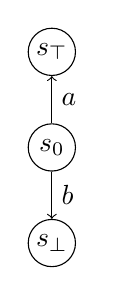
\begin{tikzpicture}	
	\node[sstate] (si) {$s_0$};
	\node[sstate,above=0.6cm of si] (s0) {$\target$};
	\node[sstate,below=0.6cm of si] (s1) {$\sink$};
	\draw[->] (si) -- node[right] {$a$} (s0);
	\draw[->] (si) -- node[right] {$b$} (s1);
	
\end{tikzpicture}
\caption{}
\end{subfigure}
\begin{subfigure}{0.38\columnwidth}
\centering
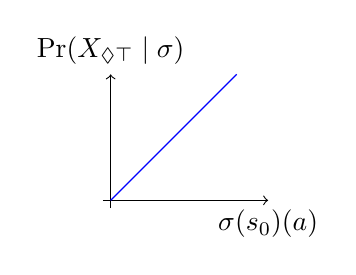
\begin{tikzpicture}[scale=2]
 \draw[->] (-0.05, 0) -- (1, 0) node[below]{$\sched(s_0)(a)$};
  	\draw[->] (0, -0.05) -- (0, 0.8) node[above] {$\Pr(X_{\lozenge\mathbf{\top}} \mid \sched)$};
  	%\draw[-,dashed] (0.4,0) -- (0.4,0.5184);
  	%\draw[-,dashed] (0.0,0.5184) -- (0.4,0.5184);
  \draw[ domain=0:0.8, smooth, variable=\x, blue] plot ({\x}, {\x});
\end{tikzpicture}
\caption{}
\end{subfigure}
\begin{subfigure}{0.38\columnwidth}
\centering
\begin{tikzpicture}[scale=2]	
 \draw[->] (-0.05, 0) -- (1, 0) node[below]{$\sched(s_0)(a)$};
  	\draw[->] (0, -0.05) -- (0, 0.8) node[above] {$H(\sched)$};
  	%\draw[-,dashed] (0.4,0) -- (0.4,0.5184);
  	%\draw[-,dashed] (0.0,0.5184) -- (0.4,0.5184);
 % \draw[ domain=0:1, smooth, variable=\x, blue] plot ({\x}, {15*(1-\x)*(1-\x)*(1-\x)*\x*\x});
\end{tikzpicture}
\caption{}
\end{subfigure}

\caption{Minimal ERCI problem.}
\end{figure}


Together, we obtain the following problem statement.
\begin{mdframed}[backgroundcolor=white!5]
\textbf{The ERCI Pareto Front Problem}:
Using the notation from the ERCI problem, find the set $\solutions \subseteq \mathbb{R}^2$.
\end{mdframed}
We are going to iteratively construct the  Pareto optimal points in $\solutions$. This yields a semi-decision procedure.
Clearly, finding $\solutions$ solves the ERCI problem, as we only need to decide whether $\langle \scthreshold, \randomness \rangle \in \solutions$.



With these facts, we are now well-equiped to develop the algorithms in Sec.~\ref{sec:mdp} for MDPs and Sec.~\ref{sec:sgs} for SGs.

Before we continue, we want to establish that Control improvisation problem is a conservative extension of deterministic case as investigated in~\cite{}.
\begin{mdframed}
\textbf{The Deterministic (Reactive) Control Improvisation (DCI) Problem~\cite{}}:
Given a \emph{deterministic} SG $\sg$, finite path sets $X_\psi$ and $X_\varphi$, and a threshold $p \in (0,1)$,  find a $\pOne$-policy $\pOneSched \in \POneScheds$  such that for every $\pTwo$-policy $\pTwoSched \in \PTwoScheds$ 
\begin{compactenum}
\item (\emph{hard constraint}) $\Pr(X_\psi \mid \sched) \geq 1$
	\item (\emph{soft constraint)} $\Pr(X_\varphi \mid \sched) \geq \scthreshold$
	\item (\emph{randomness constraint}) $\Pr(\path) \leq \delta \text{ for all } \path \in \Paths[h]{\sg[\sched]}$.
\end{compactenum}
\end{mdframed}

\begin{theorem}
	For deterministic SGs, the ERCI and DCI problem coincide.
\end{theorem}
We defer a discussion and a precise statement to Lemma~\ref{}.









\section{ERCI as multi-objective optimization}\label{sec:convex}
As may already be apparent to the reader, there is a natural trade off
between probability of generating paths in $\varphi$ (from here
onwards: \emph{the performance}) and causal entropy induced by a
policy (from here onwards: \emph{the randomization}).  In particular,
we are interested in understanding the combinations of $\scthreshold$
and $\randomness$ that allow to solve the (core) ERCI problem. To this
end, we cast ERCI as a variant of multi-objective optimization and
studying its Pareto front.

% It is convenient to consider this geometrically.
To begin, given a fixed ERCI instance, observe that a scheduler $\sched$
induces a point $x_\sched$:
\begin{equation}
  x_\sched \eqdef \Big\langle \Pr(X_\varphi \mid \sched), H(\sched) \Big\rangle \in [0,1] \times [0,\infty).  
\end{equation}
To ease notation, for $x_\sched = \langle \scp,\rndp \rangle$ we use
$\scp_\sched \eqdef \scp$ and $\rndp_\sched \eqdef \rndp$. Next, we
partially order these points via the standard product ordering:
\begin{equation}
  \langle \scp,\rndp \rangle \leq \langle \scp',\rndp' \rangle \implies \scp \leq \scp' \wedge \rndp \leq \rndp'.
\end{equation}

We say that $\pOneSched$ \emph{guarantees} a point $x_\pOne \eqdef
\langle \scp, \rndp \rangle$, if for every policy $\pTwoSched$, using
$\sched = \langle \pOneSched, \pTwoSched \rangle$, we have
$\scp_\sched \geq \scp$ and $\rndp_\sched \geq \rndp$. Thus, a point
is guaranteed if no matter what policy $\pTwo$ uses, $x_\sched$ will
induce a point no worse w.r.t.\ to either randomization or performance
than $x_\pOne$. Furthermore, observe that guaranteed points are
downward closed, i.e., if $\pOneSched$ guarantees $x$ and $x' \leq x$,
then $\pOneSched$ guarantees $x'$.

\begin{figure*}
\begin{subfigure}{0.19\textwidth}
\centering
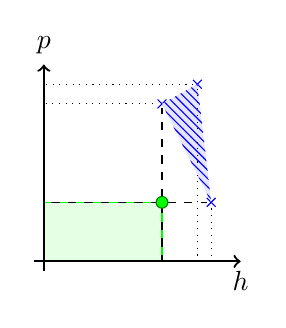
\begin{tikzpicture}[scale=2.5]	
     	
  	\draw (0.85, 0.3) node[cross=2pt,color=blue] (c1) {};
  	\draw (0.78, 0.9) node[cross=2pt,color=blue] (c2) {};
  	\draw (0.6, 0.8) node[cross=2pt,color=blue] (c3) {};
  	
  	\node at (0.6,0.3) (x1) {};
  		\draw[fill=green!10!white,draw=green] (0,0) rectangle (x1);
  		 \draw[thick, ->] (-0.05, 0) -- (1, 0) node[below]{$\rndp$};
  	\draw[thick, ->] (0, -0.05) -- (0, 1) node[above] {$\scp$};

\fill[fill=blue!10] (c1.center)--(c2.center)--(c3.center);
	
	  \fill[fill=blue!20,pattern=north west lines,pattern color=blue] (c1.center)--(c2.center)--(c3.center);
	
  	
  	\draw[dashed] (0,0) |- (c1);
  	\draw[dotted] (0,0) |- (c2);
  	\draw[dotted] (0,0) |- (c3);
  	\draw[dotted] (0,0) -| (c1);
  	\draw[dotted] (0,0) -| (c2);
  	\draw[dashed] (0,0) -| (c3);
  	
  	 
  	\draw (x1) node[circle,fill=green, inner sep=1.5pt,draw=green!50!black] {};
  
  	
  	
\end{tikzpicture}
\caption{Guaranteed points $\solutions_\pOneSched$}
\end{subfigure}
\begin{subfigure}{0.19\textwidth}
\centering
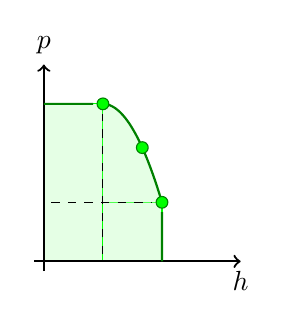
\begin{tikzpicture}[scale=2.5]	
     	
  	\node at (0.6,0.3) (x1) {};
  		\node at (0.3,0.8) (x2) {};
  	
  		\node at (0.5,0.57778) (x3) {};
  	
  		\draw[fill=green!10!white,draw=green] (0,0) rectangle (x1);
  			\draw[fill=green!10!white,draw=green] (0,0) rectangle (x2);
  			
  			
  		 \draw[thick, ->] (-0.05, 0) -- (1, 0) node[below]{$\rndp$};
  	\draw[thick, ->] (0, -0.05) -- (0, 1) node[above] {$\scp$};
  	
  
    \fill[ domain=0.3:0.6, smooth, variable=\x, green!10!white,thick] plot ({\x}, {-5.555*(\x-0.3)*(\x-0.3) + 0.8}) -- (0.3,0.3);
    
  		\draw[name path=f, domain=0.3:0.6, smooth, variable=\x, green!50!black,thick] plot ({\x}, {-5.555*(\x-0.3)*(\x-0.3) + 0.8});
    
  	
  	\draw[dashed] (0,0) -| (x1);
  	\draw[dashed] (0,0) -| (x2);
  	 \draw[dashed] (0,0) |- (x1);
  	\draw[dashed] (0,0) |- (x2);
  	
  		\draw[-,thick,color=green!50!black] (0,0.8) -- (x2);
  	\draw[-,thick,color=green!50!black] (0.6,0.0) -- (x1);
  	 
  	\draw (x1) node[circle,fill=green, inner sep=1.5pt,draw=green!50!black] {};
  \draw (x2) node[circle,fill=green, inner sep=1.5pt,draw=green!50!black] {};
  \draw (x3) node[circle,fill=green, inner sep=1.5pt,draw=green!50!black] {};
  
  
  	
  	
\end{tikzpicture}
\caption{Solutions}
\end{subfigure}
\begin{subfigure}{0.19\textwidth}
\centering
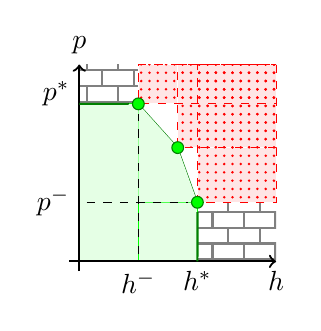
\begin{tikzpicture}[scale=2.5]	
     	
  	\node at (0.6,0.3) (x1) {};
  		\node at (0.3,0.8) (x2) {};
  	
  		\node at (0.5,0.57778) (x3) {};
  		
  					\draw[draw=none,pattern= bricks, pattern color=black!50] (1,0) rectangle (x1);
  					
  					\draw[draw=none,pattern= bricks, pattern color=black!50] (0,1) rectangle (x2);
  	
  		\draw[fill=green!10!white,draw=green] (0,0) rectangle (x1);
  			\draw[fill=green!10!white,draw=green] (0,0) rectangle (x2);
  			
  				\draw[fill=red!10!white,draw=red!0!white] (1,1) rectangle (x1);
  			\draw[fill=red!10!white,draw=red!0!white] (1,1) rectangle (x2);
  					\draw[fill=red!10!white,draw=red!0!white] (1,1) rectangle (x3);
  						\draw[draw=red,dashed] (1,1) rectangle (x1);
  			\draw[draw=red,dashed] (1,1) rectangle (x2);
  					\draw[draw= red,dashed] (1,1) rectangle (x3);
  					
  					\draw[draw=none,dashed,pattern=dots, pattern color=red] (1,1) rectangle (x1);
  					\draw[draw=none,dashed,pattern=dots, pattern color=red] (1,1) rectangle (x2);
  					\draw[draw=none,dashed,pattern=dots, pattern color=red] (1,1) rectangle (x3);
  					
  					
  			
  		 \draw[thick, ->] (-0.05, 0) -- (1, 0) node[below]{$\rndp$};
  	\draw[thick, ->] (0, -0.05) -- (0, 1) node[above] {$\scp$};
  	
  	
  	 \fill[draw=green!50!black] (x2.center) -- (x3.center) -- (x1.center);
    \fill[color=green!10!white] (x2.center) -- (x3.center) -- (x1.center) --  (0.3,0.3);
    
%  		\draw[name path=f, domain=0.3:0.6, smooth, variable=\x, green!50!black,thick] plot ({\x}, {-5.555*(\x-0.3)*(\x-0.3) + 0.8});
%    
  	
  	\draw[dashed] (0,0) -| (x1);
  	\draw[dashed] (0,0) -| (x2);
  	 \draw[dashed] (0,0) |- (x1);
  	\draw[dashed] (0,0) |- (x2);
  	
  		\draw[-,thick,color=green!50!black] (0,0.8) -- (x2);
  	\draw[-,thick,color=green!50!black] (0.6,0.0) -- (x1);
  	 
  	\draw (x1) node[circle,fill=green, inner sep=1.5pt,draw=green!50!black] {};
  \draw (x2) node[circle,fill=green, inner sep=1.5pt,draw=green!50!black] {};
  \draw (x3) node[circle,fill=green, inner sep=1.5pt,draw=green!50!black] {};
  \node[anchor=north] at (0.6,0) {$\rndopt$};
  		
  		\node[anchor=north] at (0.3,0) {$\rndmin$};
  		
  		\node[anchor=east] at (0,0.85) {$\scopt$};
  		
  		\node[anchor=east] at (0,0.3) {$\scmin$};
  
  	
  	
\end{tikzpicture}
\caption{Solutions}
\end{subfigure}
\begin{subfigure}{0.19\textwidth}
\centering
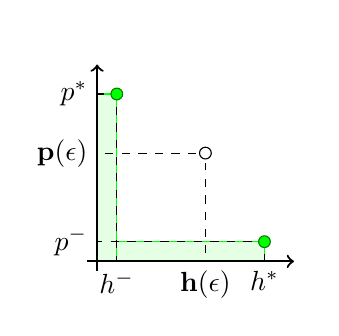
\begin{tikzpicture}[scale=2.5]	
     	
  	\node at (0.85,0.1) (x1) {};
  		\node at (0.1,0.85) (x2) {};
  		
  		\node at (0.55,0.55) (x3) {};
  		
  		\node[anchor=north] at (0.85,0) {$\rndopt$};
  		\node[anchor=north] at (0.55,0) {$\randomness(\epsilon)$};
  		
  		\node[anchor=north] at (0.1,0) {$\rndmin$};
  		
  		\node[anchor=east] at (0,0.85) {$\scopt$};
  		\node[anchor=east] at (0,0.55) {$\scthreshold(\epsilon)$};
  		
  		\node[anchor=east] at (0,0.1) {$\scmin$};
  	
  		\draw[fill=green!10!white,draw=green] (0,0) rectangle (x1);
  			\draw[fill=green!10!white,draw=green] (0,0) rectangle (x2);
  			
  		 \draw[thick, ->] (-0.05, 0) -- (1, 0) node[below]{\phantom{$\rndp$}};
  	\draw[thick, ->] (0, -0.05) -- (0, 1) node[above] {\phantom{$\scp$}};
  	
  	\draw[dashed] (0,0) -| (x1);
  	\draw[dashed] (0,0) -| (x2);
  	 \draw[dashed] (0,0) |- (x1);
  	\draw[dashed] (0,0) |- (x2);
  	
  	 \draw[dashed] (0,0) |- (x3);
  	\draw[dashed] (0,0) -| (x3);
  	 
  	\draw (x1) node[circle,fill=green, inner sep=1.5pt,draw=green!50!black] {};
  	
  	\draw (x2) node[circle,fill=green, inner sep=1.5pt,draw=green!50!black] {};
  
  	
  	
  	\draw (x3) node[circle,draw,fill=white, inner sep=1.5pt,draw=black] {};
  	
\end{tikzpicture}
\caption{Solutions}
\end{subfigure}
\begin{subfigure}{0.19\textwidth}
\centering
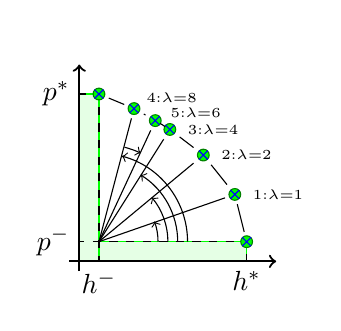
\begin{tikzpicture}[scale=2.5]	
     	
  	\node at (0.85,0.1) (x1) {};
  		\node at (0.1,0.85) (x2) {};
  		
  		
  		\node[anchor=north] at (0.85,0) {$\rndopt$};
  		
  		\node[anchor=north] at (0.1,0) {$\rndmin$};
  		
  		\node[anchor=east] at (0,0.85) {$\scopt$};
  		
  		\node[anchor=east] at (0,0.1) {$\scmin$};
  	
  		\draw[fill=green!10!white,draw=green] (0,0) rectangle (x1);
  			\draw[fill=green!10!white,draw=green] (0,0) rectangle (x2);
  			
  		 \draw[thick, ->] (-0.05, 0) -- (1, 0) node[below]{\phantom{$\rndp$}};
  	\draw[thick, ->] (0, -0.05) -- (0, 1) node[above] {\phantom{$\scp$}};
  	
  	\draw[dashed] (0,0) -| (x1);
  	\draw[dashed] (0,0) -| (x2);
  	 \draw[dashed] (0,0) |- (x1);
  	\draw[dashed] (0,0) |- (x2);
  	
  	 
  	\draw (x1) node[circle,fill=green, inner sep=1.5pt,draw=green!50!black] {};
  	
  	\draw (x2) node[circle,fill=green, inner sep=1.5pt,draw=green!50!black] {};
  	
  	\draw (x1) node[cross=2pt,color=blue] (c3) {};
  	
  	\draw (x2) node[cross=2pt,color=blue] (c3) {};
  
  \draw[black,->] (0.4,0.1) arc (0:20:0.3cm);
  
  		\node at (0.79,0.34) (x3) {};
  			\draw (x3) node[circle,fill=green, inner sep=1.5pt,draw=green!50!black] {};
  			
  	\draw (x3) node[cross=2pt,color=blue] (c3) {};
  	\draw [-] (0.1,0.1) -- (x3);
   \draw[black,->] (0.45,0.1) arc (0:40:0.35cm);
   
   \node at (0.63,0.54) (x4) {};
  			\draw (x4) node[circle,fill=green, inner sep=1.5pt,draw=green!50!black] {};
  			
  	\draw (x4) node[cross=2pt,color=blue] (c3) {};
  	\draw [-] (0.1,0.1) -- (x4);
   
   \draw[black,->] (0.5,0.1) arc (0:58:0.4cm);
    \node at (0.46,0.67) (x5) {};
  			\draw (x5) node[circle,fill=green, inner sep=1.5pt,draw=green!50!black] {};
  			
  	\draw (x5) node[cross=2pt,color=blue] (c3) {};
  	\draw [-] (0.1,0.1) -- (x5);
   \draw[black,->] (0.55,0.1) arc (0:75:0.45cm);
   \node at (0.278,0.776) (x6) {};
  			\draw (x6) node[circle,fill=green, inner sep=1.5pt,draw=green!50!black] {};
  			
  	\draw (x6) node[cross=2pt,color=blue] (c3) {};
  	\draw [-] (0.1,0.1) -- (x6);
  	
   \draw[black,->] (0.23,0.58) arc (75:65:0.5cm);
   \node at (0.386,0.715) (x7) {};
  			\draw (x7) node[circle,fill=green, inner sep=1.5pt,draw=green!50!black] {};
  			
  	\draw (x7) node[cross=2pt,color=blue] (c3) {};
  	\draw [-] (0.1,0.1) -- (x7);

   
   \draw[-] (x1) -- (x3) -- (x4) -- (x5) -- (x7) -- (x6) -- (x2);
   
   \node[anchor=west,xshift=0.3em] at (x3) {\tiny{1:$\lambda{=}1$}};
   \node[anchor=west,xshift=0.3em] at (x4) {\tiny{2:$\lambda{=}2$}};
   \node[anchor=west,xshift=0.3em] at (x5) {\tiny{3:$\lambda{=}4$}};
   \node[anchor=west,yshift=0.3em,xshift=0.2em] at (x7) {\tiny{5:$\lambda{=}6$}};
   \node[anchor=west,yshift=0.4em,xshift=0.1em] at (x6) {\tiny{4:$\lambda{=}8$}};
  	
\end{tikzpicture}
\caption{Solutions}
\end{subfigure}

\caption{Geometric interpretation of the ERCI problem for some fixed SG.}
\end{figure*}

We then define the following elementary sets: For any $\pOneSched$,
that $\pOneSched$ guarantees $\langle \scp, \rndp \rangle$, we define
the set of guaranteed points:
\begin{equation}\label{eq:guaranteed}
  \solutions[\pOneSched] \eqdef \{ \langle \scp, \rndp \rangle \mid  \pOneSched \text{ guarantees } \langle \scp, \rndp \rangle \}.
\end{equation}

Any point that can be guaranteed by some $\pOneSched$ is called
\emph{achievable}, i.e., the achievable points are: $ \solutions =
\bigcup_{\pOneSched} \solutions[\pOneSched]$.  Importantly, it holds
that the ERCI problem is satisfiable iff $\langle \scthreshold,
\randomness \rangle$ is achievable.  \sj{We should clarify satisfiable
lingo} Thus, to solve ERCI instances, we start by characterizing
$\solutions$.


\begin{proposition}
  The set of achievable points, $\solutions$, is convex. 
\end{proposition}
\begin{proof}[Proof Sketch]
  Recall that a set is convex, if it is closed under
  convex-combinations\footnotemark. Consider two points
  $\langle \scp, \rndp \rangle, \langle \scp', \rndp' \rangle \in
  \solutions$ achieved by $\pOneSched$ and $\pOneSchedPrime$
  resp. Consider the new policy, $\pi$, defined by employing
  $\pOneSched$ with probability $q$ and $\pOneSchedPrime$ with
  probability $\bar{q} \eqdef 1 - q$.  Because each policy
  \emph{guarantees} its corresponding performance, this new policy as
  performance at least $q\cdot \scp + \bar{q}\cdot \scp'$.  Similarly,
  by viewing $\pi$ as a random variable and applying chain rule
  yields,
  \begin{equation}
    \begin{split}
      H_\tau(\sigma)
      \geq &~q \cdot H( \rv{A}^{\pOne}_{1:\tau'} \mid\mid \rv{S}_{1:\tau} \mid \pi=\pOneSched)~+\\
      &~\bar{q}  \cdot H( \rv{A}^{\pOne}_{1:\tau'} \mid\mid \rv{S}_{1:\tau} \mid \pi=\pOneSchedPrime)\\
      =&~q\cdot\rndp + \bar{q}\cdot \rndp'.
    \end{split}
  \end{equation}
  Thus, any convex combination of guaranteed points is guaranteed by
  a convex combination of the resp. ego policies.
\end{proof}
\footnotetext{
  That is, $y, y' \in Y$ implies for
  every $w \in [0,1]$ that $w \cdot y + (1-w) \cdot y \in Y$
}

Next, observe that because $\solutions$ is downward closed, it
suffices to study the ``maximal'' or non-dominated points.  Precisely,
we say that a point $x$ is \emph{dominated} by $x'$, written $x \prec
x'$, if $x'$ is strictly larger in at least one dimension and not
smaller in the other, i.e., 
\begin{equation}
x \prec x' \iff x \leq x' \wedge x \neq x'.
\end{equation}
The Pareto-front $\pareto{\solutions}$ of $\solutions$ is then the set of non-dominated guaranteed points,
\begin{equation}
  \pareto{\solutions} \eqdef \{ x \in \solutions \mid \forall x' \in \solutions, x \not\prec x'  \}.  
\end{equation}
\noindent
\begin{mdframed}
Importantly, it holds that the ERCI problem is satisfiable iff there exists a  $x \in \pareto{\solutions}$ such that $\langle \scthreshold, \randomness \rangle \prec x$.    
\end{mdframed}

\noindent
Thus the approximating the Pareto-front gives a natural approximation
scheme for ERCI instances. Namely, for any subset $\pareto{} \subseteq
\pareto{\solutions}$,
\begin{enumerate}
\item If there exists an $x \in \pareto{}$ such that
$\langle \scthreshold, \randomness \rangle \prec x$, then the ERCI
Problem must be satisfiable.
\item If there exists an $x \in \pareto{}$
such that $x \prec \langle \scthreshold, \randomness \rangle$ then the
ERCI problem is not satisfiable.
\end{enumerate}

\begin{example}
	
\end{example}

Thus a key algorithmic question in ERCI is how to efficiently explore
and approximate the $\pareto{\solutions}$.  
To this end, we note that while $\solutions$ is defined as a subset of $[0,1] \times [0,\infty)$, we can restrict ourselves to the domain in which we can actually trade performance for randomness. 
We define 
$\rndopt \eqdef \max \{ \rndp \mid \exists \scp \text{ s.t. } \langle \scp, \rndp \rangle \in \solutions  \} $, i.e., the largest randomness that can be guaranteed by any $\pOne$-policy. 
Likewise, we define 
$\scopt \eqdef \max \{ \scp \mid \exists \rndp \text{ s.t. } \langle \scp, \rndp \rangle \in \solutions  \} $, i.e., the largest performance that can be guaranteed by any $\pOne$-policy. 
Then, we define 
$\scmin \eqdef \max \{ \scp \mid \langle \scp, \rndopt \rangle  \in \solutions \}$, the best performance that $\pOne$ can guarantee while guaranteeing optimal randomness. 
Likewise, we define  the analogous $\rndmin \eqdef \max \{ \scp \mid \langle \scp, \rndopt \rangle  \in \solutions \}$.
We thus obtain two points on the Pareto-curve: $\langle \scmin, \rndopt \rangle$ and $\langle \scopt, \rndmin \rangle$, and intuitively, we can trade between these two points following the Pareto curve.

\begin{remark}[Regret Based ERCI]
  In practice, rather that fixing $\scthreshold$ and $\randomness$ a
  priori, one seeks achieve some percentage of the achievable soft
  constraint or causal entropy measure.  In such cases, we
  re-parameterized the ERCI instance with:
  \begin{equation}
    \scthreshold(\epsilon) \eqdef \epsilon \cdot \scopt
    \hspace{3em}
    \randomness(\delta) \eqdef  \delta \cdot \rndopt
  \end{equation}
  where $\epsilon, \delta \in [0, 1]$. As we shall later see, these maximum quantities are
  directly computed in our proposed algorithm.
\end{remark}

Finally, it is helpful to think about the Pareto-curve as a function
in $\rndp$.  We define a characteristic function which given a target
performance ratio, $\epsilon$, yields the optimal randomness ratio,
$\delta$:
\begin{equation}
  \begin{split}
    & \solfuncp\colon [0,1] \rightarrow [0, 1]    \\
    & \solfuncp(\delta) = \max_\epsilon \{ \rndp(\delta) \mid \langle
    \scp(\epsilon), \rndp(\delta) \rangle \in \solutions \} 
  \end{split}
\end{equation}
\begin{proposition}\label{prop:monotone}
  $\solfuncp$ is smooth and (strictly) monotonically decreasing.
\end{proposition}
In particular, the set is \emph{not} a finite polytope, but can be
well approximated by one. We shall however post-pone the proof of
\propref{monotone} until Sec ?. For now, one case observe that
(non-strict) monotone decreasing follows directly from convexity and
using the adequate domains.


With these facts, we are now well-equiped to develop the algorithms in Sec.~\ref{sec:mdps} for MDPs and Sec.~\ref{sec:sgs} for SGs.

%%% Local Variables:
%%% mode: latex
%%% TeX-master: "main"
%%% End:



\section{The Control Improvisation Problem for MDPs}
\label{sec:mdps}

We present an algorithm for the control improvisation problem for
MDPs, which in the next section, will serve as a subroutine for an
algorithm on SGs. Our goal shall be to instantiate the approximation
scheme from the previous section. In particular, we seek
to find points on the Pareto curve $\pareto{\solutions}$ and
incrementally build up $\pareto{} \subseteq \pareto{\solutions}$.
\subsection{Rationality}
To start, recall that an MDP is a stochastic game with no action
choices for the environment, i.e., the environment is purely
stochastic and the only degree of freedom is $\pOne$'s policy.  The
key idea for finding points on the Pareto-curve is to rephrase the
trade-off between randomization and performance as a degree in
rationality $\rat$ of the policy.  Formally, the rationality
corresponds to the following scalarization of our multi-objective
problem~\cite{DBLP:journals/corr/abs-1805-00909},
\begin{equation}
  \label{eq:scalarization}
  J_\rat(\sched) \eqdef \Big\langle 1, \rat\Big\rangle \cdot \Big\langle\rndp_\sched, \scp_\sched\Big\rangle.
\end{equation}
In context of MDPs, the \textbf{unique} ($\pOne$-)policy that
optimizes~\eqref{eq:scalarization} is given by a smooth variant of the
Bellman equations~\cite{mceThesis, DBLP:conf/cav/Vazquez-Chanlatte20}. Namely, let $\smoothmax{}$ denote
the log-sum-exp operator, i.e.,
$\smoothmax(X) \eqdef \log \left( \sum_{x\in X} e^x \right)$. For each
rationality $\rat \in [0, \infty)$, we define a policy $\sched_\rat$
-- using $s = \last{\path}$ -- as follows:
 \begin{align}
   &\sched_\rat(\act \mid s) \eqdef \exp( Q_\rat(s,\act) - V_\rat(s))  \label{eq:mdp:first}\\
   & V_\rat(s) \eqdef  \begin{cases}
     \lambda  \cdot \indicator{s = \target} & \text{if }s \in \{ \target, \sink \},\\
     \smoothmax_{\act \in \EnAct(s)}{  Q_\rat(s,\act) } & \text{otherwise.}
   \end{cases}\label{eq:mdp:v}\\ 
	& Q_\rat(s, \act) \eqdef \sum_{s'} P(s,\act,s') \cdot V_\rat(s').\label{eq:mdp:last}
 \end{align}
To ease notation, we denote $x_\rat \eqdef x_{\sched_\rat},
\scp_\rat \eqdef \scp_{\sched_\rat}, \rndp_\rat \eqdef
\rndp_{\sched_\rat}$. 
 % As previously alluded at the start of the subsection, the key property
% is that $\sched_\rat$ is the \emph{unique} maximum causal entropy policy
% such that $\Pr(\varphi) = \scp_\rat$~\cite{mceThesis}.
Intuitively, as $\rat \rightarrow 0$, $\sched_\rat$ approaches the
uniform distribution over \emph{all available actions}. Note that this
policy maximizes (causal) entropy, and thus $\rndopt = \rndp_0$.  As
$\lambda \rightarrow \infty$, this variant of the Bellman equations
coincides with the standard Bellman
equations~\cite{DBLP:books/wi/Puterman94}, where $\sched_\rat$ selects
(uniformly) from actions \emph{that maximize performance}.
Furthermore, the monotonicity and smoothness of the above Bellman
equations yields the following proposition.
\begin{proposition}
  $\scp_\rat$ is  continuously (and strictly) increasing in $\rat$ and $\rndp_\rat$
  is smoothly (and strictly) decreasing in $\rat$.
\end{proposition}
\noindent In terms of $\solfuncp$, we can define:
\begin{equation}
  \epsilon_\rat \eqdef \frac{\scp_\rat - \scp_0}{\scp_\infty} + \scp_0
  \hspace{1em}\text{and}\hspace{1em}
\delta_\rat \eqdef \frac{\rndp_\rat - \rndp_\infty}{\rndp_0} +
\rndp_{\infty}. 
\end{equation}

Then, because $\sched_\rat$ maximizes randomness
given a target performance, one derives:
\begin{equation}
  \solfuncp\left(\delta_\rat\right) = \epsilon_\rat.
\end{equation}

What remains is to instantiate the approximation scheme for the Pareto
front by varying the optimization direction
$\langle \rat, 1\rangle$.\footnote{Assuming $\scopt, \rndopt \neq 0$
  (which would otherwise yield trivial $\solutions$ and
  $\pareto{\solutions}$)}  In particular, we construct
$\pareto{} = \{ x_\rat \mid \rat \in \{ \rat_1, \rat_2, \hdots \} \}$
until $\pareto{}$ contains a witness to either realizability or
unrealizability of the ERCI instance. We notice that the scalarization in \eqref{eq:scalarization} means that we may additionally exploit witnesses to unrealizability as outlined in Remark~\ref{rem:scalarwitnesses}. In the remainder of this
section, we improve upon randomly selecting values for $\rat$.



%
%and by varying $\rat$ we can explore the Pareto front. First observe the following easily verified proposition.
%\begin{proposition}
%  $\scp_\rat$ is smoothly and (strictly) monotonically increasing in $\rat$ and $\rndp_\rat$
%  is smoothly (strictly) monotonically decreasing in $\rat$.
%\end{proposition}

\subsection{Targeted Pareto-exploration}
The key ingredient to improve upon arbitrarily selecting $\rat_1, \hdots \rat_i$ is to exploit additional structure of the rationality.  
%The key algorithmic idea is thus to strategically evaluate a sequence
%of rationality coefficients to yield (input, output) pairs for
%$\solfuncp$. Due to convexity, the convex hull this sequence of
%rationality-indexed points (and the origin) gradually refines a
%polygonal approximation of $\solutions$, and thus the Pareto
%Front. This approximation, $\hat{\solutions}$, is refined until
%either:
%\begin{enumerate}
%\item $\langle \scthreshold, \randomness \rangle \in \hat{\solutions}$ proving
%  $\langle \scthreshold, \randomness \rangle \in \solutions$.
%\item A $\rat$ is found such that
%  $x_{\rat} \prec \langle \scthreshold, \randomness \rangle$, proving
%  $\langle \scthreshold, \randomness \rangle \notin \solutions$.
%\end{enumerate}
%
%
%Next, to extract an improviser, observe that because
%$\hat{\solutions}$ is a convex polygon, if $\langle \scthreshold,
%\randomness \rangle \in \hat{S}$, then there must two corners of
%$\hat{\solutions}$ indexed by $\rat_1$ and $\rat_2$, that form a
%triangle with $(0, 0)$ containing $\langle \scthreshold, \randomness
%\rangle$. Thus, as in the convexity proof, there must be a convex
%combination of $q\cdot x_{\rat_1} + \bar{q}\cdot x_{\rat_2}$ that
%dominates $\langle \scthreshold, \randomness \rangle$. Therefore, the
%following policy solves the ERCI instance:

%\mypara{Approximation Sequence} 
%The final algorithmic question for
%MDPs is then: what order should one evaluate rationality coefficients.
We propose a three staged sequence: (i) Compute $x_\rat$ for the end
points $\rat \in \{0, \infty\}$.  (ii) Double $\rat$ (starting at $\lambda=1$) until $h_\rat \leq
\randomness$, yielding $\rat_1\ldots \rat_j$.
(iii) Binary search for $\rat \in [\rat_{j-1}, \rat_{j}]$. We illustrate the idea in Fig.~\ref{fig:geom:doubling}.

The algorithm terminates almost surely, that is: 
the algorithm halts if $\langle \scthreshold, \randomness \rangle$ is
not on $\pareto{\solutions}$ (or if we happen to exactly hit $\langle \scthreshold, \randomness\rangle$ by selecting some rationality $\rat$).
As the Pareto front has
measure 0, we argue that not halting is thus merely a technical concern, as a
small perturbation to the ERCI instance (i.e. a \emph{smoothed
analysis}~\cite{SmoothedAnalysis}) on $\sg$ admits decidability. 
\begin{mdframed}
  Our approximation scheme yields a semi-decision process which halts
  iff either (a) $\langle \scthreshold, \randomness \rangle$ is
  bounded away from $\pareto{\solutions}$ \emph{or} (b)
  $\langle \scthreshold, \randomness \rangle$ is dominated by
  $x_{\rat_i}$.
\end{mdframed}
Next, observe that if we terminate the binary search when the search
region is smaller than $\Delta$, this approximation scheme becomes linear in the MDP size
and logarithmic in the final rationality, $\rat_*$, and the
resolution, $\Delta$, i.e., the run-time is,
\begin{equation}
  \mathcal{O}\Big(~\hspace{-1.4em}\underbrace{|\sg|}_{\text{Evaluate $x_\rat$}}\hspace{-1.4em}~\cdot\overbrace{\log(\rat_*)}^{\text{Doubling Phase}}\cdot\underbrace{\log(\nicefrac{1}{\Delta})}_{\text{Binary Search}}\Big)
\end{equation}
Finally, before generalizing to stochastic games, we observe that in
practice, $\rat = 100$ yields a nearly optimal policy, and thus one
can often assume $\rat_* \leq 100$ in our run-time analysis.

%%% Local Variables:
%%% mode: latex
%%% TeX-master: "main"
%%% End:

 
\section{The Control Improvisation Problem for SGs}\label{sec:sgs}

MDP algorithm in hand, we are now ready to provide an algorithm for
stochastic games.
%At a high level, this algorithm works by initially
%planning for $\pTwo$ selecting the action that minimizes randomness
%(with ties broken by performance). This assumption leads to a
%reduction to the MDP-case, where the rationality indexed family,
%$\sched_\rat$, indexes the Pareto Front.  If this assumption is ever
%violated, the resulting state must support more randomness.  The
%rationality, $\rat$, is thus lowered to match the worst case randomness,
%which due to monotonicity of $\solfuncp$, can only increase
%performance. Surprisingly, as we shall later prove, this class of
%policies indexes the Pareto Front for SGs!


\begin{figure}
\centering
\scalebox{0.8}{
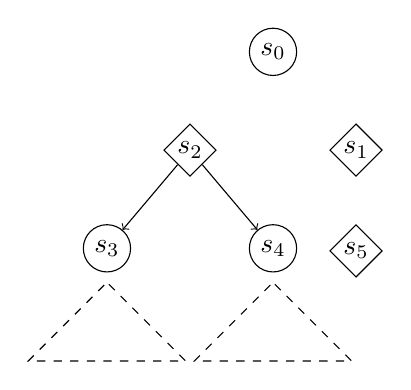
\begin{tikzpicture}
    \node[sstate] (a1) {$s_0$}; 
    
	\node[astate,below=0.6cm of a1,xshift=3em] (a2) {$s_1$};
	\node[astate,below=0.6cm of a2] (a3) {$s_5$};
	
	\node[astate,below=0.6cm of a1,xshift=-3em] (a0) {$s_2$};
	\node[sstate,below=0.6cm of a0,xshift=-3em] (s1) {$s_3$};
	\node[sstate,below=0.6cm  of a0,xshift=3em] (s2) {$s_4$};
	
	\node[below=0.1cm of s1, inner sep=0.3pt] (x1) {};
	
	\node[below=0.1cm of s2, inner sep=0.3pt] (x2) {};
	
	\draw[->] (a0) -- (s1);
	\draw[->] (a0) -- (s2);
	
	\draw[dashed] (x1) -- +(1,-1) -- +(-1,-1) -- (x1);
	\draw[dashed] (x2) -- +(1,-1) -- +(-1,-1)  -- (x2);
	
	
\end{tikzpicture}
}
\caption{Simple SG to illustrate intuition {\color{red}WIP}}
\label{fig:sg:simplest}
\end{figure}
\sj{Update figure}

\mypara{Intuition}
Before we discuss the algorithm in full detail, we consider two simple cases with a single $\pTwo$-state: First, the simplest class of true 2-player SGs, with an initial $\pTwo$-state and two independent MDPs with only $\pOne$-states, as illustrated in the dashed Fig.~\ref{fig:sg:simplest} and assuming that $s_2$ is the initial state.
For both MDP subgames, we can compute (an approximation of) the Pareto front and the corresponding sets of achievable solutions as described in Section~\ref{sec:mdps}. 
The achievable points for the SG are now given by the intersection of the two points. 
However, the challenge in this generalization is to select action for $\pOne$-states.
Therefore, consider the full SG illustrated in Fig.~\ref{fig:sg:simplest} with initial state $s_0$. 
To determine $\pOneSched(s_0)$, we must plan for whatever action $\pTwo$ selects in $s_2$ and optimally without calculating all Pareto-fronts a priori. 
What our algorithm, roughly, does is to assume that in the $\pTwo$-node, $\pTwo$ aims to minimize entropy and we compute the maximal entropy of its successors ($\pOne$-states). Under this assumption, for a required randomness $\delta$ we can compute the required rationality $\rat$ to solve the overall ERCI problem. The $\pOne$-policy memorizes this rationality. Now, whenever $\pTwo$ diverges from minimizing maximal entropy, the idea is that $\pOne$ can play with higher rationality and still ensure the same randomness $\delta$. We call the increase in rationality \emph{replanning}.
By traversing the graph top-down using this idea (and memoizing the visited state-rationality pairs $s,\rat$), we can explore how we can optimize performance while always matching the required randomness.  In the remainder of this section, we formalize and analyze this algorithmic idea.

\mypara{Environment Policies}
We make some observations about the $\pTwo$-policies. 
For the purpose of ERCI, we can assume an adversarial policy that aims to disprove that we can meet the performance \emph{and} randomization requirement. 
To do so, it suffices to violate either performance \emph{or} randomization. 
Furthermore, if there is a violating $\pTwo$-policy, there is a deterministic $\pTwo$-policy that proves this. 
In particular, in every state,  $\pTwoSched$ may thus aim to disprove either objective by choosing the appropriate action, and there is no incentive to randomize.
%Finally, these responses can be computed via a standard dynamic programming (topologically from terminal states to the initial state) operation. 

%First and foremost, observe that to render an ERCI instance
%un-achievable, it suffices for $\pTwo$ to violate
%either the performance threshold \emph{or} the randomness threshold.  Next,
%notice that because $\pOneSched$ is a priori fixed, $\pTwoSched$ can
%be seen as repeatedly selecting between a convex combination of
%$\rndp$ (and $\scp$) for the corresponding sub-graph. As the maximum of a
%convex combination is always achievable on the boundaries, we can
%w.l.o.g. assume that $\pTwoSched$ is \emph{deterministic}.  Similarly,
%notice that given a fixed $\pOneSched$, the worst-case $\pTwoSched$
%response can be computed via dynamic programming in topological order
%from the leafs to the root of $\sg$.

\mypara{Counter-policies}
First, assume $\rat$ is also a priori fixed.  
Again, via dynamic programming, we can compute the
$\pTwo$ policy that minimizes the maximal causal entropy, denoted $\sched_\rat^\pTwo$.
In particular, we use the following update of \eqref{eq:mdp:v} to the SG case:
 \begin{align}
   & V_\rat(s) \eqdef  \begin{cases}
     \lambda  \cdot \indicator{s = \target} & \text{if }s \in \{ \target, \sink \},\\
     \smoothmax_{\act \in \EnAct(s)}{  Q_\rat(s,\act) } & \text{if } s \in S_\pOne. \\
     \min_{\act \in \EnAct(s)}{  Q_\rat(s,\act) } &  \text{if } s \in S_\pTwo.
   \end{cases}
 \end{align}

Second, suppose $\pTwoSched$ was fixed, than the SG reduces to 
a MDP that we denote $\sg[\pTwoSched]$.
For every $\rat$, the policy in the SG that correspond to the policy $\sched_\lambda$ in $\sg[\pTwoSched]$ is denoted $\sched^\pOne_\rat[\pTwoSched]$.
The latter (set\footnote{These policies are no longer unique because some parts of the SG may be unreachable under $\pTwoSched$} of) policies can be thought of as the counter-policies that $\pOne$ uses to maximize entropy against a fixed $\pTwoSched$. 
Together, for fixed $\rat$, we can compute the scheduler of the $\pTwo$-scheduler that minimizes maximal entropy and its counterstrategy as: $\pi_\rat \eqdef \langle
\sched^\pOne_\rat[\sched_\rat^\pTwo] , \sched_\rat^\pTwo \rangle$.
%
%On the other hand, suppose $\pTwoSched$ was known, reducing the SG to
%a MDP. As discussed in the previous section, for the MDP case, it
%suffices to consider rationality indexed policies. Let use denote the
%resulting MDP and maximum causal entropy family of (partial) policies
%as $\sg[\pTwoSched]$ and $\pi^\pOne_\rat[\pTwoSched]$ resp. Now
%suppose $\rat$ is a priori fixed. Again, via a topological ordered
%evaluation of states from the leaves to the root, one can compute the
%$\pTwo$ policy, call $\sched_\rat^\pTwo$, that minimizes the maximum
%causal entropy policy family, $\pi^\pOne_\rat[~.~]$. By
%We shall refer to resulting (partial) schedule as: $\pi_\rat \eqdef \langle
%\pi^\pOne_\rat[\sched_\rat^\pTwo] , \sched_\rat^\pTwo \rangle$.

\mypara{Replanning}
Of course, even if $\rat$ is fixed, $\pTwoSched$ need not be
$\sched^\pTwo_\rat$. Nevertheless,  by selecting the worst
entropy MDP, $\pi_\rat$ establishes an achievable randomness for the
sub-game rooted at each state, call $\delta_\rat(s)$. Now suppose,
$\pTwo$ deviates from $\sched_\rat^\pTwo$ at state $s$. Note that, so
long as $\pOneSched$  yield randomness less than
$\delta_\rat(s)$ at the new successor-state, the worst-case randomness will not decrease.
This begs the question ``what maximum performance can $\pOne$ guarantee at $s' \in
\Succ(s)$ given randomness $\delta_\rat(s)$?'' This question can be investigated on a sub-game, and eventually, must be answered on an MDP. 
\begin{mdframed}
  The key observation is that each state $s'$ is the root of a sub
  game, $\sg[s]$, with a corresponding Pareto Front,
  $\pareto{\solutions}[s]$.
\end{mdframed}
In particular, given access the characteristic functions,
$f_\solutions^{s'}$, for each $s' \in \Succ(s)$, one can compute:
\begin{equation}\label{eq:performance_lookup}
  \epsilon_\rat(s) = \min_{s'} f_\solutions^{s'}(\delta_\rat(s)).
\end{equation}
Thus, via dynamic programming, one can define $\epsilon_\rat(\iota)$.
Moreover, assuming that this entropy matching family of policies
indexes $\pareto{\solutions}$ (proved in~Sec.~\ref{sec:proofs}), one can handle
deviations from $\sigma^\pTwo_\rat$ by ``replanning''. Namely, one
extends $\pi_\rat$ at $s'$ by computing a new rationality coefficient,
$\rat'$, such that:
\begin{equation}
  \delta_{\rat'}(s') = \delta_{\rat}(s)
\end{equation}
Due to the monotonicity $\rat \leq \rat'$, and thus $\epsilon_\rat \leq \epsilon_{\rat'}$, 
Therefore, ignoring the feasibility of computing the exact Pareto
Front, we obtain a synthesis algorithm for SGs!

\mypara{Approximate Pareto Fronts}
Of course, by varying $\rat$, one can only construct approximate
Pareto fronts $\pareto{} \subseteq \pareto{\solutions}$, where we denote the downward closure of $\pareto{}$ as $\hat{\solutions} \subseteq \solutions$.
 %let $\hat{f}_\solutions^{s'}$ denote the characterising function.
    We now
adapt the above algorithm to the case where $\hat{\solutions}$ is a $\kappa$-close approximation of $\solutions$, where $\kappa$ bounds the $\infty$-norm
error. In particular, for such an approximation, the performance from state  $s$ for fixed rationality $\rat$, $\epsilon_\rat(s)$, is bounded up to  $\kappa$. 
Convex combinations of these intervals cannot
increase the error beyond $\kappa$, i.e.,
\begin{equation}
  q\cdot[x, x + \kappa] + \bar{q}\cdot[y, y + \kappa] = [z, z + \kappa],
\end{equation}
where $z = q\cdot x + \bar{q}\cdot y$. \sj{Sentences from here are vague}Thus, since $\pi_\rat$ and
$P(s, a)$ are independent of this Pareto front (and manipulate
performance via convex combinations) the error can only accumulate on
the Pareto Fronts for $s \in S_\pTwo$. Notice then that so long as,
$\kappa\cdot\tau$\sj{what is $\tau$ doing here} is enough resolution to answer $\scp_\rat <
\scthreshold$, one obtains a semi-decision procedure as in the MDP
case.\sj{We have not talked about $\scthreshold$ in this section at all...}
We propose the following high-level algorithm:
\begin{mdframed}
\begin{enumerate}
\item Let $0 < \kappa < 1$ be some arbitrary initial tolerance.
\item Recursively compute $\kappa$-close Pareto fronts for each successor state using replanning.
\item If $\scthreshold$ is within $\kappa\cdot \tau$ distance to (but outside of) $\hat{\pareto{\solutions}}$,
  halve $\kappa$ and repeat.
\end{enumerate}  
\end{mdframed}
\sj{Symmary has new symbols, and what si $\tau$ doing there?}
\mypara{Termination and Run Time}
First, the algorithm halts almost surely, that is: 
the algorithm halts if $\langle \scthreshold, \randomness \rangle$ is
not on $\pareto{\solutions}$ (or if we happen to exactly hit $\langle \scthreshold, \randomness\rangle$ by selecting some rationality $\rat$).
As the Pareto Front has
measure 0, we argue that not halting is thus merely a technical concern, as a
small perturbation to the ERCI instance (i.e. a \emph{smoothed
analysis}~\cite{SmoothedAnalysis}) on $\sg$ admits decidability. 
The same observation hold also for the MDP case.

While for practical run time, the algorithm can be significantly improved by adaptive
tolerances, lazily computing the Pareto Fronts, and only computing
Pareto Fronts for $\pTwo$ states.
We give an output-sensitive analysis of the run time (assuming it does halt) in the naive formulation.
 If $\kappa^*$ tolerance is required to terminate,
then the $\kappa$ search introduces $\mathcal{O}(\log(\nicefrac{1}{\kappa^*}))$
iterations. Furthermore, by computing $\mathcal{O}(|\sg|)$ Pareto fronts, one ensures that the complexity grows linearly with the graph
size - although the multiplicative constant depends on the number of
rationality coefficients explored per Pareto front. We found that most
of the rationality coefficients explored were shared, which in
practice seems to amortize the cost per state. 

%In practice, this algorithm can be significantly improved by adaptive
%tolerances, lazily computing the Pareto Fronts, and only computing
%Pareto Fronts for $\pTwo$ states. Nevertheless,
%already this na\"ive algorithm gives a sense of the run-time
%bottlenecks. Namely, if $\kappa^*$ tolerance is required to terminate,
%then the $\kappa$ search introduces $O(\log(\nicefrac{1}{\kappa^*}))$
%iterations. Furthermore, by computing $O(|\sg|)$ Pareto fronts, from the
%leaves, one ensures that the complexity grows linearly with the graph
%size - although the multiplicative constant depends on the number of
%rationality coefficients explored per Pareto front. We found that most
%of the rationality coefficients explored were shared, which in
%practice seems to amortize the cost per state. Finally, as in the
%MDP-case, the algorithm halts if $\langle \scthreshold, \randomness \rangle$ is
%bounded away from the root Pareto Front. As the Pareto Front has
%measure 0, we argue that this is merely a technical concern, as a
%small perturbation to the ERCI instance (i.e. a Smoothed
%Analysis~\cite{SmoothedAnalysis}) on $\sg$ admits decidability.

\mypara{On Completeness}
Our algorithm restricts itself to considering only recursive entropy
matching policies, $\{\sched^{\pOne}_\rat\}_\rat$.  Importantly,
observe that because fixing a policy yields a verifiable point in
$\solutions$, any witness for satisfiability we find is trivially sound. We can restrict ourselves to the case in which our
algorithm claims the ERCI instance unsatisfiable. Surprisingly, the class of policies we consider suffices, and the algorithm 
is thus sound and (whenever halting) complete (proof provided in Sec~\ref{sec:proofs}).

Finally, observe that as a corollary of the entropy matching family
$\{\sched^{\pOne}_\rat\}_\rat$ being complete, it must be the case that
$\solfuncp(\rndp_\rat)$ inherits continuity and (strict) monotonicity
from the MDP case. Namely, at each $\pTwo$ state, the achievable
points $\solutions$ are necessarily the intersection of the achievable
points of the subgraphs. By induction, (with the MDP base case), we
obtain continuity and strict monotonicity.


%%% Local Variables:
%%% mode: latex
%%% TeX-master: "main"
%%% End:

%\begin{mdframed}
%
%\begin{compactenum}
%	\item $\Pr^\sg_{\langle \sched_1,\sched_2 \rangle}(\eventually{h} T) \geq 1$
%	\item $\Pr^\sg_{\langle \sched_1,\sched_2 \rangle}(\eventually{h} G) \geq \lambda$ 
%\end{compactenum}
%\end{mdframed}
%\sj{Define randomly selected policy}
%\sj{Describe in terms of pMDPp}


\section{Implementation and Empirical Evaluation}
\label{sec:empirical}
\begin{figure*}
  \begin{subfigure}{0.5\textwidth}
  \centering
  \scalebox{0.58}{
    %% Creator: Matplotlib, PGF backend
%%
%% To include the figure in your LaTeX document, write
%%   \input{<filename>.pgf}
%%
%% Make sure the required packages are loaded in your preamble
%%   \usepackage{pgf}
%%
%% and, on pdftex
%%   \usepackage[utf8]{inputenc}\DeclareUnicodeCharacter{2212}{-}
%%
%% or, on luatex and xetex
%%   \usepackage{unicode-math}
%%
%% Figures using additional raster images can only be included by \input if
%% they are in the same directory as the main LaTeX file. For loading figures
%% from other directories you can use the `import` package
%%   \usepackage{import}
%%
%% and then include the figures with
%%   \import{<path to file>}{<filename>.pgf}
%%
%% Matplotlib used the following preamble
%%   \usepackage{fontspec}
%%   \setmainfont{DejaVuSerif.ttf}[Path=/home/mvc/.cache/pypoetry/virtualenvs/improvisers-CRyZdLN2-py3.8/lib/python3.8/site-packages/matplotlib/mpl-data/fonts/ttf/]
%%   \setsansfont{DejaVuSans.ttf}[Path=/home/mvc/.cache/pypoetry/virtualenvs/improvisers-CRyZdLN2-py3.8/lib/python3.8/site-packages/matplotlib/mpl-data/fonts/ttf/]
%%   \setmonofont{DejaVuSansMono.ttf}[Path=/home/mvc/.cache/pypoetry/virtualenvs/improvisers-CRyZdLN2-py3.8/lib/python3.8/site-packages/matplotlib/mpl-data/fonts/ttf/]
%%
\begingroup%
\makeatletter%
\begin{pgfpicture}%
\pgfpathrectangle{\pgfpointorigin}{\pgfqpoint{6.000000in}{4.000000in}}%
\pgfusepath{use as bounding box, clip}%
\begin{pgfscope}%
\pgfsetbuttcap%
\pgfsetmiterjoin%
\definecolor{currentfill}{rgb}{1.000000,1.000000,1.000000}%
\pgfsetfillcolor{currentfill}%
\pgfsetlinewidth{0.000000pt}%
\definecolor{currentstroke}{rgb}{1.000000,1.000000,1.000000}%
\pgfsetstrokecolor{currentstroke}%
\pgfsetstrokeopacity{0.000000}%
\pgfsetdash{}{0pt}%
\pgfpathmoveto{\pgfqpoint{0.000000in}{0.000000in}}%
\pgfpathlineto{\pgfqpoint{6.000000in}{0.000000in}}%
\pgfpathlineto{\pgfqpoint{6.000000in}{4.000000in}}%
\pgfpathlineto{\pgfqpoint{0.000000in}{4.000000in}}%
\pgfpathclose%
\pgfusepath{fill}%
\end{pgfscope}%
\begin{pgfscope}%
\pgfsetbuttcap%
\pgfsetmiterjoin%
\definecolor{currentfill}{rgb}{1.000000,1.000000,1.000000}%
\pgfsetfillcolor{currentfill}%
\pgfsetlinewidth{0.000000pt}%
\definecolor{currentstroke}{rgb}{0.000000,0.000000,0.000000}%
\pgfsetstrokecolor{currentstroke}%
\pgfsetstrokeopacity{0.000000}%
\pgfsetdash{}{0pt}%
\pgfpathmoveto{\pgfqpoint{0.750000in}{0.500000in}}%
\pgfpathlineto{\pgfqpoint{5.400000in}{0.500000in}}%
\pgfpathlineto{\pgfqpoint{5.400000in}{3.520000in}}%
\pgfpathlineto{\pgfqpoint{0.750000in}{3.520000in}}%
\pgfpathclose%
\pgfusepath{fill}%
\end{pgfscope}%
\begin{pgfscope}%
\pgfpathrectangle{\pgfqpoint{0.750000in}{0.500000in}}{\pgfqpoint{4.650000in}{3.020000in}}%
\pgfusepath{clip}%
\pgfsetroundcap%
\pgfsetroundjoin%
\pgfsetlinewidth{0.803000pt}%
\definecolor{currentstroke}{rgb}{0.800000,0.800000,0.800000}%
\pgfsetstrokecolor{currentstroke}%
\pgfsetdash{}{0pt}%
\pgfpathmoveto{\pgfqpoint{0.960047in}{0.500000in}}%
\pgfpathlineto{\pgfqpoint{0.960047in}{3.520000in}}%
\pgfusepath{stroke}%
\end{pgfscope}%
\begin{pgfscope}%
\definecolor{textcolor}{rgb}{0.150000,0.150000,0.150000}%
\pgfsetstrokecolor{textcolor}%
\pgfsetfillcolor{textcolor}%
\pgftext[x=0.960047in,y=0.402778in,,top]{\color{textcolor}\sffamily\fontsize{10.000000}{12.000000}\selectfont 0}%
\end{pgfscope}%
\begin{pgfscope}%
\pgfpathrectangle{\pgfqpoint{0.750000in}{0.500000in}}{\pgfqpoint{4.650000in}{3.020000in}}%
\pgfusepath{clip}%
\pgfsetroundcap%
\pgfsetroundjoin%
\pgfsetlinewidth{0.803000pt}%
\definecolor{currentstroke}{rgb}{0.800000,0.800000,0.800000}%
\pgfsetstrokecolor{currentstroke}%
\pgfsetdash{}{0pt}%
\pgfpathmoveto{\pgfqpoint{1.874112in}{0.500000in}}%
\pgfpathlineto{\pgfqpoint{1.874112in}{3.520000in}}%
\pgfusepath{stroke}%
\end{pgfscope}%
\begin{pgfscope}%
\definecolor{textcolor}{rgb}{0.150000,0.150000,0.150000}%
\pgfsetstrokecolor{textcolor}%
\pgfsetfillcolor{textcolor}%
\pgftext[x=1.874112in,y=0.402778in,,top]{\color{textcolor}\sffamily\fontsize{10.000000}{12.000000}\selectfont 50000}%
\end{pgfscope}%
\begin{pgfscope}%
\pgfpathrectangle{\pgfqpoint{0.750000in}{0.500000in}}{\pgfqpoint{4.650000in}{3.020000in}}%
\pgfusepath{clip}%
\pgfsetroundcap%
\pgfsetroundjoin%
\pgfsetlinewidth{0.803000pt}%
\definecolor{currentstroke}{rgb}{0.800000,0.800000,0.800000}%
\pgfsetstrokecolor{currentstroke}%
\pgfsetdash{}{0pt}%
\pgfpathmoveto{\pgfqpoint{2.788176in}{0.500000in}}%
\pgfpathlineto{\pgfqpoint{2.788176in}{3.520000in}}%
\pgfusepath{stroke}%
\end{pgfscope}%
\begin{pgfscope}%
\definecolor{textcolor}{rgb}{0.150000,0.150000,0.150000}%
\pgfsetstrokecolor{textcolor}%
\pgfsetfillcolor{textcolor}%
\pgftext[x=2.788176in,y=0.402778in,,top]{\color{textcolor}\sffamily\fontsize{10.000000}{12.000000}\selectfont 100000}%
\end{pgfscope}%
\begin{pgfscope}%
\pgfpathrectangle{\pgfqpoint{0.750000in}{0.500000in}}{\pgfqpoint{4.650000in}{3.020000in}}%
\pgfusepath{clip}%
\pgfsetroundcap%
\pgfsetroundjoin%
\pgfsetlinewidth{0.803000pt}%
\definecolor{currentstroke}{rgb}{0.800000,0.800000,0.800000}%
\pgfsetstrokecolor{currentstroke}%
\pgfsetdash{}{0pt}%
\pgfpathmoveto{\pgfqpoint{3.702240in}{0.500000in}}%
\pgfpathlineto{\pgfqpoint{3.702240in}{3.520000in}}%
\pgfusepath{stroke}%
\end{pgfscope}%
\begin{pgfscope}%
\definecolor{textcolor}{rgb}{0.150000,0.150000,0.150000}%
\pgfsetstrokecolor{textcolor}%
\pgfsetfillcolor{textcolor}%
\pgftext[x=3.702240in,y=0.402778in,,top]{\color{textcolor}\sffamily\fontsize{10.000000}{12.000000}\selectfont 150000}%
\end{pgfscope}%
\begin{pgfscope}%
\pgfpathrectangle{\pgfqpoint{0.750000in}{0.500000in}}{\pgfqpoint{4.650000in}{3.020000in}}%
\pgfusepath{clip}%
\pgfsetroundcap%
\pgfsetroundjoin%
\pgfsetlinewidth{0.803000pt}%
\definecolor{currentstroke}{rgb}{0.800000,0.800000,0.800000}%
\pgfsetstrokecolor{currentstroke}%
\pgfsetdash{}{0pt}%
\pgfpathmoveto{\pgfqpoint{4.616304in}{0.500000in}}%
\pgfpathlineto{\pgfqpoint{4.616304in}{3.520000in}}%
\pgfusepath{stroke}%
\end{pgfscope}%
\begin{pgfscope}%
\definecolor{textcolor}{rgb}{0.150000,0.150000,0.150000}%
\pgfsetstrokecolor{textcolor}%
\pgfsetfillcolor{textcolor}%
\pgftext[x=4.616304in,y=0.402778in,,top]{\color{textcolor}\sffamily\fontsize{10.000000}{12.000000}\selectfont 200000}%
\end{pgfscope}%
\begin{pgfscope}%
\definecolor{textcolor}{rgb}{0.150000,0.150000,0.150000}%
\pgfsetstrokecolor{textcolor}%
\pgfsetfillcolor{textcolor}%
\pgftext[x=3.075000in,y=0.212809in,,top]{\color{textcolor}\sffamily\fontsize{10.000000}{12.000000}\selectfont BDD nodes ($\approx$ 2 $\times$ game states)}%
\end{pgfscope}%
\begin{pgfscope}%
\pgfpathrectangle{\pgfqpoint{0.750000in}{0.500000in}}{\pgfqpoint{4.650000in}{3.020000in}}%
\pgfusepath{clip}%
\pgfsetroundcap%
\pgfsetroundjoin%
\pgfsetlinewidth{0.803000pt}%
\definecolor{currentstroke}{rgb}{0.800000,0.800000,0.800000}%
\pgfsetstrokecolor{currentstroke}%
\pgfsetdash{}{0pt}%
\pgfpathmoveto{\pgfqpoint{0.750000in}{0.636333in}}%
\pgfpathlineto{\pgfqpoint{5.400000in}{0.636333in}}%
\pgfusepath{stroke}%
\end{pgfscope}%
\begin{pgfscope}%
\definecolor{textcolor}{rgb}{0.150000,0.150000,0.150000}%
\pgfsetstrokecolor{textcolor}%
\pgfsetfillcolor{textcolor}%
\pgftext[x=0.564412in, y=0.583571in, left, base]{\color{textcolor}\sffamily\fontsize{10.000000}{12.000000}\selectfont 0}%
\end{pgfscope}%
\begin{pgfscope}%
\pgfpathrectangle{\pgfqpoint{0.750000in}{0.500000in}}{\pgfqpoint{4.650000in}{3.020000in}}%
\pgfusepath{clip}%
\pgfsetroundcap%
\pgfsetroundjoin%
\pgfsetlinewidth{0.803000pt}%
\definecolor{currentstroke}{rgb}{0.800000,0.800000,0.800000}%
\pgfsetstrokecolor{currentstroke}%
\pgfsetdash{}{0pt}%
\pgfpathmoveto{\pgfqpoint{0.750000in}{1.267896in}}%
\pgfpathlineto{\pgfqpoint{5.400000in}{1.267896in}}%
\pgfusepath{stroke}%
\end{pgfscope}%
\begin{pgfscope}%
\definecolor{textcolor}{rgb}{0.150000,0.150000,0.150000}%
\pgfsetstrokecolor{textcolor}%
\pgfsetfillcolor{textcolor}%
\pgftext[x=0.387682in, y=1.215134in, left, base]{\color{textcolor}\sffamily\fontsize{10.000000}{12.000000}\selectfont 100}%
\end{pgfscope}%
\begin{pgfscope}%
\pgfpathrectangle{\pgfqpoint{0.750000in}{0.500000in}}{\pgfqpoint{4.650000in}{3.020000in}}%
\pgfusepath{clip}%
\pgfsetroundcap%
\pgfsetroundjoin%
\pgfsetlinewidth{0.803000pt}%
\definecolor{currentstroke}{rgb}{0.800000,0.800000,0.800000}%
\pgfsetstrokecolor{currentstroke}%
\pgfsetdash{}{0pt}%
\pgfpathmoveto{\pgfqpoint{0.750000in}{1.899459in}}%
\pgfpathlineto{\pgfqpoint{5.400000in}{1.899459in}}%
\pgfusepath{stroke}%
\end{pgfscope}%
\begin{pgfscope}%
\definecolor{textcolor}{rgb}{0.150000,0.150000,0.150000}%
\pgfsetstrokecolor{textcolor}%
\pgfsetfillcolor{textcolor}%
\pgftext[x=0.387682in, y=1.846698in, left, base]{\color{textcolor}\sffamily\fontsize{10.000000}{12.000000}\selectfont 200}%
\end{pgfscope}%
\begin{pgfscope}%
\pgfpathrectangle{\pgfqpoint{0.750000in}{0.500000in}}{\pgfqpoint{4.650000in}{3.020000in}}%
\pgfusepath{clip}%
\pgfsetroundcap%
\pgfsetroundjoin%
\pgfsetlinewidth{0.803000pt}%
\definecolor{currentstroke}{rgb}{0.800000,0.800000,0.800000}%
\pgfsetstrokecolor{currentstroke}%
\pgfsetdash{}{0pt}%
\pgfpathmoveto{\pgfqpoint{0.750000in}{2.531023in}}%
\pgfpathlineto{\pgfqpoint{5.400000in}{2.531023in}}%
\pgfusepath{stroke}%
\end{pgfscope}%
\begin{pgfscope}%
\definecolor{textcolor}{rgb}{0.150000,0.150000,0.150000}%
\pgfsetstrokecolor{textcolor}%
\pgfsetfillcolor{textcolor}%
\pgftext[x=0.387682in, y=2.478261in, left, base]{\color{textcolor}\sffamily\fontsize{10.000000}{12.000000}\selectfont 300}%
\end{pgfscope}%
\begin{pgfscope}%
\pgfpathrectangle{\pgfqpoint{0.750000in}{0.500000in}}{\pgfqpoint{4.650000in}{3.020000in}}%
\pgfusepath{clip}%
\pgfsetroundcap%
\pgfsetroundjoin%
\pgfsetlinewidth{0.803000pt}%
\definecolor{currentstroke}{rgb}{0.800000,0.800000,0.800000}%
\pgfsetstrokecolor{currentstroke}%
\pgfsetdash{}{0pt}%
\pgfpathmoveto{\pgfqpoint{0.750000in}{3.162586in}}%
\pgfpathlineto{\pgfqpoint{5.400000in}{3.162586in}}%
\pgfusepath{stroke}%
\end{pgfscope}%
\begin{pgfscope}%
\definecolor{textcolor}{rgb}{0.150000,0.150000,0.150000}%
\pgfsetstrokecolor{textcolor}%
\pgfsetfillcolor{textcolor}%
\pgftext[x=0.387682in, y=3.109824in, left, base]{\color{textcolor}\sffamily\fontsize{10.000000}{12.000000}\selectfont 400}%
\end{pgfscope}%
\begin{pgfscope}%
\definecolor{textcolor}{rgb}{0.150000,0.150000,0.150000}%
\pgfsetstrokecolor{textcolor}%
\pgfsetfillcolor{textcolor}%
\pgftext[x=0.332126in,y=2.010000in,,bottom,rotate=90.000000]{\color{textcolor}\sffamily\fontsize{10.000000}{12.000000}\selectfont Time to approximate Pareto Front (sec)}%
\end{pgfscope}%
\begin{pgfscope}%
\pgfpathrectangle{\pgfqpoint{0.750000in}{0.500000in}}{\pgfqpoint{4.650000in}{3.020000in}}%
\pgfusepath{clip}%
\pgfsetbuttcap%
\pgfsetroundjoin%
\definecolor{currentfill}{rgb}{0.121569,0.466667,0.705882}%
\pgfsetfillcolor{currentfill}%
\pgfsetfillopacity{0.200000}%
\pgfsetlinewidth{1.003750pt}%
\definecolor{currentstroke}{rgb}{0.121569,0.466667,0.705882}%
\pgfsetstrokecolor{currentstroke}%
\pgfsetstrokeopacity{0.200000}%
\pgfsetdash{}{0pt}%
\pgfsys@defobject{currentmarker}{\pgfqpoint{0.961364in}{0.637273in}}{\pgfqpoint{0.964197in}{0.639408in}}{%
\pgfpathmoveto{\pgfqpoint{0.961364in}{0.637295in}}%
\pgfpathlineto{\pgfqpoint{0.961364in}{0.637273in}}%
\pgfpathlineto{\pgfqpoint{0.964197in}{0.639401in}}%
\pgfpathlineto{\pgfqpoint{0.964197in}{0.639408in}}%
\pgfpathlineto{\pgfqpoint{0.964197in}{0.639408in}}%
\pgfpathlineto{\pgfqpoint{0.961364in}{0.637295in}}%
\pgfpathclose%
\pgfusepath{stroke,fill}%
}%
\begin{pgfscope}%
\pgfsys@transformshift{0.000000in}{0.000000in}%
\pgfsys@useobject{currentmarker}{}%
\end{pgfscope}%
\end{pgfscope}%
\begin{pgfscope}%
\pgfpathrectangle{\pgfqpoint{0.750000in}{0.500000in}}{\pgfqpoint{4.650000in}{3.020000in}}%
\pgfusepath{clip}%
\pgfsetbuttcap%
\pgfsetroundjoin%
\definecolor{currentfill}{rgb}{1.000000,0.498039,0.054902}%
\pgfsetfillcolor{currentfill}%
\pgfsetfillopacity{0.200000}%
\pgfsetlinewidth{1.003750pt}%
\definecolor{currentstroke}{rgb}{1.000000,0.498039,0.054902}%
\pgfsetstrokecolor{currentstroke}%
\pgfsetstrokeopacity{0.200000}%
\pgfsetdash{}{0pt}%
\pgfsys@defobject{currentmarker}{\pgfqpoint{0.961364in}{0.639248in}}{\pgfqpoint{0.964197in}{0.640187in}}{%
\pgfpathmoveto{\pgfqpoint{0.961364in}{0.639755in}}%
\pgfpathlineto{\pgfqpoint{0.961364in}{0.639248in}}%
\pgfpathlineto{\pgfqpoint{0.964197in}{0.639667in}}%
\pgfpathlineto{\pgfqpoint{0.964197in}{0.640187in}}%
\pgfpathlineto{\pgfqpoint{0.964197in}{0.640187in}}%
\pgfpathlineto{\pgfqpoint{0.961364in}{0.639755in}}%
\pgfpathclose%
\pgfusepath{stroke,fill}%
}%
\begin{pgfscope}%
\pgfsys@transformshift{0.000000in}{0.000000in}%
\pgfsys@useobject{currentmarker}{}%
\end{pgfscope}%
\end{pgfscope}%
\begin{pgfscope}%
\pgfpathrectangle{\pgfqpoint{0.750000in}{0.500000in}}{\pgfqpoint{4.650000in}{3.020000in}}%
\pgfusepath{clip}%
\pgfsetbuttcap%
\pgfsetroundjoin%
\definecolor{currentfill}{rgb}{0.121569,0.466667,0.705882}%
\pgfsetfillcolor{currentfill}%
\pgfsetlinewidth{0.481800pt}%
\definecolor{currentstroke}{rgb}{1.000000,1.000000,1.000000}%
\pgfsetstrokecolor{currentstroke}%
\pgfsetdash{}{0pt}%
\pgfsys@defobject{currentmarker}{\pgfqpoint{-0.041667in}{-0.041667in}}{\pgfqpoint{0.041667in}{0.041667in}}{%
\pgfpathmoveto{\pgfqpoint{0.000000in}{-0.041667in}}%
\pgfpathcurveto{\pgfqpoint{0.011050in}{-0.041667in}}{\pgfqpoint{0.021649in}{-0.037276in}}{\pgfqpoint{0.029463in}{-0.029463in}}%
\pgfpathcurveto{\pgfqpoint{0.037276in}{-0.021649in}}{\pgfqpoint{0.041667in}{-0.011050in}}{\pgfqpoint{0.041667in}{0.000000in}}%
\pgfpathcurveto{\pgfqpoint{0.041667in}{0.011050in}}{\pgfqpoint{0.037276in}{0.021649in}}{\pgfqpoint{0.029463in}{0.029463in}}%
\pgfpathcurveto{\pgfqpoint{0.021649in}{0.037276in}}{\pgfqpoint{0.011050in}{0.041667in}}{\pgfqpoint{0.000000in}{0.041667in}}%
\pgfpathcurveto{\pgfqpoint{-0.011050in}{0.041667in}}{\pgfqpoint{-0.021649in}{0.037276in}}{\pgfqpoint{-0.029463in}{0.029463in}}%
\pgfpathcurveto{\pgfqpoint{-0.037276in}{0.021649in}}{\pgfqpoint{-0.041667in}{0.011050in}}{\pgfqpoint{-0.041667in}{0.000000in}}%
\pgfpathcurveto{\pgfqpoint{-0.041667in}{-0.011050in}}{\pgfqpoint{-0.037276in}{-0.021649in}}{\pgfqpoint{-0.029463in}{-0.029463in}}%
\pgfpathcurveto{\pgfqpoint{-0.021649in}{-0.037276in}}{\pgfqpoint{-0.011050in}{-0.041667in}}{\pgfqpoint{0.000000in}{-0.041667in}}%
\pgfpathclose%
\pgfusepath{stroke,fill}%
}%
\begin{pgfscope}%
\pgfsys@transformshift{1.105219in}{0.754121in}%
\pgfsys@useobject{currentmarker}{}%
\end{pgfscope}%
\begin{pgfscope}%
\pgfsys@transformshift{1.201013in}{0.828556in}%
\pgfsys@useobject{currentmarker}{}%
\end{pgfscope}%
\begin{pgfscope}%
\pgfsys@transformshift{1.313607in}{0.925811in}%
\pgfsys@useobject{currentmarker}{}%
\end{pgfscope}%
\begin{pgfscope}%
\pgfsys@transformshift{1.435946in}{1.018527in}%
\pgfsys@useobject{currentmarker}{}%
\end{pgfscope}%
\begin{pgfscope}%
\pgfsys@transformshift{1.564116in}{1.129954in}%
\pgfsys@useobject{currentmarker}{}%
\end{pgfscope}%
\begin{pgfscope}%
\pgfsys@transformshift{1.699434in}{1.259082in}%
\pgfsys@useobject{currentmarker}{}%
\end{pgfscope}%
\begin{pgfscope}%
\pgfsys@transformshift{1.838628in}{1.394207in}%
\pgfsys@useobject{currentmarker}{}%
\end{pgfscope}%
\begin{pgfscope}%
\pgfsys@transformshift{1.981130in}{1.531734in}%
\pgfsys@useobject{currentmarker}{}%
\end{pgfscope}%
\begin{pgfscope}%
\pgfsys@transformshift{0.973283in}{0.652078in}%
\pgfsys@useobject{currentmarker}{}%
\end{pgfscope}%
\begin{pgfscope}%
\pgfsys@transformshift{0.988621in}{0.666943in}%
\pgfsys@useobject{currentmarker}{}%
\end{pgfscope}%
\begin{pgfscope}%
\pgfsys@transformshift{1.032478in}{0.719431in}%
\pgfsys@useobject{currentmarker}{}%
\end{pgfscope}%
\begin{pgfscope}%
\pgfsys@transformshift{1.095512in}{0.723893in}%
\pgfsys@useobject{currentmarker}{}%
\end{pgfscope}%
\begin{pgfscope}%
\pgfsys@transformshift{1.199404in}{0.782613in}%
\pgfsys@useobject{currentmarker}{}%
\end{pgfscope}%
\begin{pgfscope}%
\pgfsys@transformshift{1.326624in}{0.877374in}%
\pgfsys@useobject{currentmarker}{}%
\end{pgfscope}%
\begin{pgfscope}%
\pgfsys@transformshift{1.484958in}{0.955615in}%
\pgfsys@useobject{currentmarker}{}%
\end{pgfscope}%
\begin{pgfscope}%
\pgfsys@transformshift{1.659124in}{1.100753in}%
\pgfsys@useobject{currentmarker}{}%
\end{pgfscope}%
\begin{pgfscope}%
\pgfsys@transformshift{2.235935in}{1.438964in}%
\pgfsys@useobject{currentmarker}{}%
\end{pgfscope}%
\begin{pgfscope}%
\pgfsys@transformshift{3.220876in}{2.113420in}%
\pgfsys@useobject{currentmarker}{}%
\end{pgfscope}%
\begin{pgfscope}%
\pgfsys@transformshift{4.204537in}{2.739110in}%
\pgfsys@useobject{currentmarker}{}%
\end{pgfscope}%
\begin{pgfscope}%
\pgfsys@transformshift{5.188636in}{3.382727in}%
\pgfsys@useobject{currentmarker}{}%
\end{pgfscope}%
\begin{pgfscope}%
\pgfsys@transformshift{0.961364in}{0.637273in}%
\pgfsys@useobject{currentmarker}{}%
\end{pgfscope}%
\begin{pgfscope}%
\pgfsys@transformshift{0.964197in}{0.639401in}%
\pgfsys@useobject{currentmarker}{}%
\end{pgfscope}%
\begin{pgfscope}%
\pgfsys@transformshift{0.974124in}{0.644823in}%
\pgfsys@useobject{currentmarker}{}%
\end{pgfscope}%
\begin{pgfscope}%
\pgfsys@transformshift{0.993246in}{0.653992in}%
\pgfsys@useobject{currentmarker}{}%
\end{pgfscope}%
\begin{pgfscope}%
\pgfsys@transformshift{1.036719in}{0.676435in}%
\pgfsys@useobject{currentmarker}{}%
\end{pgfscope}%
\begin{pgfscope}%
\pgfsys@transformshift{1.102916in}{0.722829in}%
\pgfsys@useobject{currentmarker}{}%
\end{pgfscope}%
\begin{pgfscope}%
\pgfsys@transformshift{1.207868in}{0.776134in}%
\pgfsys@useobject{currentmarker}{}%
\end{pgfscope}%
\begin{pgfscope}%
\pgfsys@transformshift{1.351230in}{0.883244in}%
\pgfsys@useobject{currentmarker}{}%
\end{pgfscope}%
\begin{pgfscope}%
\pgfsys@transformshift{0.961364in}{0.637295in}%
\pgfsys@useobject{currentmarker}{}%
\end{pgfscope}%
\begin{pgfscope}%
\pgfsys@transformshift{0.964197in}{0.639408in}%
\pgfsys@useobject{currentmarker}{}%
\end{pgfscope}%
\begin{pgfscope}%
\pgfsys@transformshift{0.974106in}{0.644281in}%
\pgfsys@useobject{currentmarker}{}%
\end{pgfscope}%
\begin{pgfscope}%
\pgfsys@transformshift{0.991930in}{0.653801in}%
\pgfsys@useobject{currentmarker}{}%
\end{pgfscope}%
\begin{pgfscope}%
\pgfsys@transformshift{1.034617in}{0.751047in}%
\pgfsys@useobject{currentmarker}{}%
\end{pgfscope}%
\begin{pgfscope}%
\pgfsys@transformshift{1.098126in}{0.718782in}%
\pgfsys@useobject{currentmarker}{}%
\end{pgfscope}%
\begin{pgfscope}%
\pgfsys@transformshift{1.207887in}{0.784511in}%
\pgfsys@useobject{currentmarker}{}%
\end{pgfscope}%
\begin{pgfscope}%
\pgfsys@transformshift{1.363918in}{0.896800in}%
\pgfsys@useobject{currentmarker}{}%
\end{pgfscope}%
\end{pgfscope}%
\begin{pgfscope}%
\pgfpathrectangle{\pgfqpoint{0.750000in}{0.500000in}}{\pgfqpoint{4.650000in}{3.020000in}}%
\pgfusepath{clip}%
\pgfsetbuttcap%
\pgfsetroundjoin%
\definecolor{currentfill}{rgb}{1.000000,0.498039,0.054902}%
\pgfsetfillcolor{currentfill}%
\pgfsetlinewidth{0.481800pt}%
\definecolor{currentstroke}{rgb}{1.000000,1.000000,1.000000}%
\pgfsetstrokecolor{currentstroke}%
\pgfsetdash{}{0pt}%
\pgfsys@defobject{currentmarker}{\pgfqpoint{-0.041667in}{-0.041667in}}{\pgfqpoint{0.041667in}{0.041667in}}{%
\pgfpathmoveto{\pgfqpoint{0.000000in}{-0.041667in}}%
\pgfpathcurveto{\pgfqpoint{0.011050in}{-0.041667in}}{\pgfqpoint{0.021649in}{-0.037276in}}{\pgfqpoint{0.029463in}{-0.029463in}}%
\pgfpathcurveto{\pgfqpoint{0.037276in}{-0.021649in}}{\pgfqpoint{0.041667in}{-0.011050in}}{\pgfqpoint{0.041667in}{0.000000in}}%
\pgfpathcurveto{\pgfqpoint{0.041667in}{0.011050in}}{\pgfqpoint{0.037276in}{0.021649in}}{\pgfqpoint{0.029463in}{0.029463in}}%
\pgfpathcurveto{\pgfqpoint{0.021649in}{0.037276in}}{\pgfqpoint{0.011050in}{0.041667in}}{\pgfqpoint{0.000000in}{0.041667in}}%
\pgfpathcurveto{\pgfqpoint{-0.011050in}{0.041667in}}{\pgfqpoint{-0.021649in}{0.037276in}}{\pgfqpoint{-0.029463in}{0.029463in}}%
\pgfpathcurveto{\pgfqpoint{-0.037276in}{0.021649in}}{\pgfqpoint{-0.041667in}{0.011050in}}{\pgfqpoint{-0.041667in}{0.000000in}}%
\pgfpathcurveto{\pgfqpoint{-0.041667in}{-0.011050in}}{\pgfqpoint{-0.037276in}{-0.021649in}}{\pgfqpoint{-0.029463in}{-0.029463in}}%
\pgfpathcurveto{\pgfqpoint{-0.021649in}{-0.037276in}}{\pgfqpoint{-0.011050in}{-0.041667in}}{\pgfqpoint{0.000000in}{-0.041667in}}%
\pgfpathclose%
\pgfusepath{stroke,fill}%
}%
\begin{pgfscope}%
\pgfsys@transformshift{1.105219in}{0.639249in}%
\pgfsys@useobject{currentmarker}{}%
\end{pgfscope}%
\begin{pgfscope}%
\pgfsys@transformshift{1.201013in}{0.639280in}%
\pgfsys@useobject{currentmarker}{}%
\end{pgfscope}%
\begin{pgfscope}%
\pgfsys@transformshift{1.313607in}{0.644556in}%
\pgfsys@useobject{currentmarker}{}%
\end{pgfscope}%
\begin{pgfscope}%
\pgfsys@transformshift{1.435946in}{0.640370in}%
\pgfsys@useobject{currentmarker}{}%
\end{pgfscope}%
\begin{pgfscope}%
\pgfsys@transformshift{1.564116in}{0.640938in}%
\pgfsys@useobject{currentmarker}{}%
\end{pgfscope}%
\begin{pgfscope}%
\pgfsys@transformshift{1.699434in}{0.663616in}%
\pgfsys@useobject{currentmarker}{}%
\end{pgfscope}%
\begin{pgfscope}%
\pgfsys@transformshift{1.838628in}{0.642346in}%
\pgfsys@useobject{currentmarker}{}%
\end{pgfscope}%
\begin{pgfscope}%
\pgfsys@transformshift{1.981130in}{0.643110in}%
\pgfsys@useobject{currentmarker}{}%
\end{pgfscope}%
\begin{pgfscope}%
\pgfsys@transformshift{0.973283in}{0.638892in}%
\pgfsys@useobject{currentmarker}{}%
\end{pgfscope}%
\begin{pgfscope}%
\pgfsys@transformshift{0.988621in}{0.639338in}%
\pgfsys@useobject{currentmarker}{}%
\end{pgfscope}%
\begin{pgfscope}%
\pgfsys@transformshift{1.032478in}{0.639662in}%
\pgfsys@useobject{currentmarker}{}%
\end{pgfscope}%
\begin{pgfscope}%
\pgfsys@transformshift{1.095512in}{0.640149in}%
\pgfsys@useobject{currentmarker}{}%
\end{pgfscope}%
\begin{pgfscope}%
\pgfsys@transformshift{1.199404in}{0.640916in}%
\pgfsys@useobject{currentmarker}{}%
\end{pgfscope}%
\begin{pgfscope}%
\pgfsys@transformshift{1.326624in}{0.641421in}%
\pgfsys@useobject{currentmarker}{}%
\end{pgfscope}%
\begin{pgfscope}%
\pgfsys@transformshift{1.484958in}{0.642190in}%
\pgfsys@useobject{currentmarker}{}%
\end{pgfscope}%
\begin{pgfscope}%
\pgfsys@transformshift{1.659124in}{0.643622in}%
\pgfsys@useobject{currentmarker}{}%
\end{pgfscope}%
\begin{pgfscope}%
\pgfsys@transformshift{2.235935in}{0.646218in}%
\pgfsys@useobject{currentmarker}{}%
\end{pgfscope}%
\begin{pgfscope}%
\pgfsys@transformshift{3.220876in}{0.667886in}%
\pgfsys@useobject{currentmarker}{}%
\end{pgfscope}%
\begin{pgfscope}%
\pgfsys@transformshift{4.204537in}{0.661769in}%
\pgfsys@useobject{currentmarker}{}%
\end{pgfscope}%
\begin{pgfscope}%
\pgfsys@transformshift{5.188636in}{0.675696in}%
\pgfsys@useobject{currentmarker}{}%
\end{pgfscope}%
\begin{pgfscope}%
\pgfsys@transformshift{0.961364in}{0.639248in}%
\pgfsys@useobject{currentmarker}{}%
\end{pgfscope}%
\begin{pgfscope}%
\pgfsys@transformshift{0.964197in}{0.639667in}%
\pgfsys@useobject{currentmarker}{}%
\end{pgfscope}%
\begin{pgfscope}%
\pgfsys@transformshift{0.974124in}{0.640085in}%
\pgfsys@useobject{currentmarker}{}%
\end{pgfscope}%
\begin{pgfscope}%
\pgfsys@transformshift{0.993246in}{0.640643in}%
\pgfsys@useobject{currentmarker}{}%
\end{pgfscope}%
\begin{pgfscope}%
\pgfsys@transformshift{1.036719in}{0.641578in}%
\pgfsys@useobject{currentmarker}{}%
\end{pgfscope}%
\begin{pgfscope}%
\pgfsys@transformshift{1.102916in}{0.642000in}%
\pgfsys@useobject{currentmarker}{}%
\end{pgfscope}%
\begin{pgfscope}%
\pgfsys@transformshift{1.207868in}{0.643092in}%
\pgfsys@useobject{currentmarker}{}%
\end{pgfscope}%
\begin{pgfscope}%
\pgfsys@transformshift{1.351230in}{0.644432in}%
\pgfsys@useobject{currentmarker}{}%
\end{pgfscope}%
\begin{pgfscope}%
\pgfsys@transformshift{0.961364in}{0.639755in}%
\pgfsys@useobject{currentmarker}{}%
\end{pgfscope}%
\begin{pgfscope}%
\pgfsys@transformshift{0.964197in}{0.640187in}%
\pgfsys@useobject{currentmarker}{}%
\end{pgfscope}%
\begin{pgfscope}%
\pgfsys@transformshift{0.974106in}{0.640811in}%
\pgfsys@useobject{currentmarker}{}%
\end{pgfscope}%
\begin{pgfscope}%
\pgfsys@transformshift{0.991930in}{0.641331in}%
\pgfsys@useobject{currentmarker}{}%
\end{pgfscope}%
\begin{pgfscope}%
\pgfsys@transformshift{1.034617in}{0.642092in}%
\pgfsys@useobject{currentmarker}{}%
\end{pgfscope}%
\begin{pgfscope}%
\pgfsys@transformshift{1.098126in}{0.642681in}%
\pgfsys@useobject{currentmarker}{}%
\end{pgfscope}%
\begin{pgfscope}%
\pgfsys@transformshift{1.207887in}{0.644420in}%
\pgfsys@useobject{currentmarker}{}%
\end{pgfscope}%
\begin{pgfscope}%
\pgfsys@transformshift{1.363918in}{0.645614in}%
\pgfsys@useobject{currentmarker}{}%
\end{pgfscope}%
\end{pgfscope}%
\begin{pgfscope}%
\pgfpathrectangle{\pgfqpoint{0.750000in}{0.500000in}}{\pgfqpoint{4.650000in}{3.020000in}}%
\pgfusepath{clip}%
\pgfsetroundcap%
\pgfsetroundjoin%
\pgfsetlinewidth{1.505625pt}%
\definecolor{currentstroke}{rgb}{0.121569,0.466667,0.705882}%
\pgfsetstrokecolor{currentstroke}%
\pgfsetdash{}{0pt}%
\pgfpathmoveto{\pgfqpoint{0.961364in}{0.637284in}}%
\pgfpathlineto{\pgfqpoint{0.964197in}{0.639405in}}%
\pgfpathlineto{\pgfqpoint{0.973283in}{0.652078in}}%
\pgfpathlineto{\pgfqpoint{0.974106in}{0.644281in}}%
\pgfpathlineto{\pgfqpoint{0.974124in}{0.644823in}}%
\pgfpathlineto{\pgfqpoint{0.988621in}{0.666943in}}%
\pgfpathlineto{\pgfqpoint{0.991930in}{0.653801in}}%
\pgfpathlineto{\pgfqpoint{0.993246in}{0.653992in}}%
\pgfpathlineto{\pgfqpoint{1.032478in}{0.719431in}}%
\pgfpathlineto{\pgfqpoint{1.034617in}{0.751047in}}%
\pgfpathlineto{\pgfqpoint{1.036719in}{0.676435in}}%
\pgfpathlineto{\pgfqpoint{1.095512in}{0.723893in}}%
\pgfpathlineto{\pgfqpoint{1.098126in}{0.718782in}}%
\pgfpathlineto{\pgfqpoint{1.102916in}{0.722829in}}%
\pgfpathlineto{\pgfqpoint{1.105219in}{0.754121in}}%
\pgfpathlineto{\pgfqpoint{1.199404in}{0.782613in}}%
\pgfpathlineto{\pgfqpoint{1.201013in}{0.828556in}}%
\pgfpathlineto{\pgfqpoint{1.207868in}{0.776134in}}%
\pgfpathlineto{\pgfqpoint{1.207887in}{0.784511in}}%
\pgfpathlineto{\pgfqpoint{1.313607in}{0.925811in}}%
\pgfpathlineto{\pgfqpoint{1.326624in}{0.877374in}}%
\pgfpathlineto{\pgfqpoint{1.351230in}{0.883244in}}%
\pgfpathlineto{\pgfqpoint{1.363918in}{0.896800in}}%
\pgfpathlineto{\pgfqpoint{1.435946in}{1.018527in}}%
\pgfpathlineto{\pgfqpoint{1.484958in}{0.955615in}}%
\pgfpathlineto{\pgfqpoint{1.564116in}{1.129954in}}%
\pgfpathlineto{\pgfqpoint{1.659124in}{1.100753in}}%
\pgfpathlineto{\pgfqpoint{1.699434in}{1.259082in}}%
\pgfpathlineto{\pgfqpoint{1.838628in}{1.394207in}}%
\pgfpathlineto{\pgfqpoint{1.981130in}{1.531734in}}%
\pgfpathlineto{\pgfqpoint{2.235935in}{1.438964in}}%
\pgfpathlineto{\pgfqpoint{3.220876in}{2.113420in}}%
\pgfpathlineto{\pgfqpoint{4.204537in}{2.739110in}}%
\pgfpathlineto{\pgfqpoint{5.188636in}{3.382727in}}%
\pgfusepath{stroke}%
\end{pgfscope}%
\begin{pgfscope}%
\pgfpathrectangle{\pgfqpoint{0.750000in}{0.500000in}}{\pgfqpoint{4.650000in}{3.020000in}}%
\pgfusepath{clip}%
\pgfsetroundcap%
\pgfsetroundjoin%
\pgfsetlinewidth{1.505625pt}%
\definecolor{currentstroke}{rgb}{1.000000,0.498039,0.054902}%
\pgfsetstrokecolor{currentstroke}%
\pgfsetdash{}{0pt}%
\pgfpathmoveto{\pgfqpoint{0.961364in}{0.639501in}}%
\pgfpathlineto{\pgfqpoint{0.964197in}{0.639927in}}%
\pgfpathlineto{\pgfqpoint{0.973283in}{0.638892in}}%
\pgfpathlineto{\pgfqpoint{0.974106in}{0.640811in}}%
\pgfpathlineto{\pgfqpoint{0.974124in}{0.640085in}}%
\pgfpathlineto{\pgfqpoint{0.988621in}{0.639338in}}%
\pgfpathlineto{\pgfqpoint{0.991930in}{0.641331in}}%
\pgfpathlineto{\pgfqpoint{0.993246in}{0.640643in}}%
\pgfpathlineto{\pgfqpoint{1.032478in}{0.639662in}}%
\pgfpathlineto{\pgfqpoint{1.034617in}{0.642092in}}%
\pgfpathlineto{\pgfqpoint{1.036719in}{0.641578in}}%
\pgfpathlineto{\pgfqpoint{1.095512in}{0.640149in}}%
\pgfpathlineto{\pgfqpoint{1.098126in}{0.642681in}}%
\pgfpathlineto{\pgfqpoint{1.102916in}{0.642000in}}%
\pgfpathlineto{\pgfqpoint{1.105219in}{0.639249in}}%
\pgfpathlineto{\pgfqpoint{1.199404in}{0.640916in}}%
\pgfpathlineto{\pgfqpoint{1.201013in}{0.639280in}}%
\pgfpathlineto{\pgfqpoint{1.207868in}{0.643092in}}%
\pgfpathlineto{\pgfqpoint{1.207887in}{0.644420in}}%
\pgfpathlineto{\pgfqpoint{1.313607in}{0.644556in}}%
\pgfpathlineto{\pgfqpoint{1.326624in}{0.641421in}}%
\pgfpathlineto{\pgfqpoint{1.351230in}{0.644432in}}%
\pgfpathlineto{\pgfqpoint{1.363918in}{0.645614in}}%
\pgfpathlineto{\pgfqpoint{1.435946in}{0.640370in}}%
\pgfpathlineto{\pgfqpoint{1.484958in}{0.642190in}}%
\pgfpathlineto{\pgfqpoint{1.564116in}{0.640938in}}%
\pgfpathlineto{\pgfqpoint{1.659124in}{0.643622in}}%
\pgfpathlineto{\pgfqpoint{1.699434in}{0.663616in}}%
\pgfpathlineto{\pgfqpoint{1.838628in}{0.642346in}}%
\pgfpathlineto{\pgfqpoint{1.981130in}{0.643110in}}%
\pgfpathlineto{\pgfqpoint{2.235935in}{0.646218in}}%
\pgfpathlineto{\pgfqpoint{3.220876in}{0.667886in}}%
\pgfpathlineto{\pgfqpoint{4.204537in}{0.661769in}}%
\pgfpathlineto{\pgfqpoint{5.188636in}{0.675696in}}%
\pgfusepath{stroke}%
\end{pgfscope}%
\begin{pgfscope}%
\pgfsetrectcap%
\pgfsetmiterjoin%
\pgfsetlinewidth{0.803000pt}%
\definecolor{currentstroke}{rgb}{0.800000,0.800000,0.800000}%
\pgfsetstrokecolor{currentstroke}%
\pgfsetdash{}{0pt}%
\pgfpathmoveto{\pgfqpoint{0.750000in}{0.500000in}}%
\pgfpathlineto{\pgfqpoint{0.750000in}{3.520000in}}%
\pgfusepath{stroke}%
\end{pgfscope}%
\begin{pgfscope}%
\pgfsetrectcap%
\pgfsetmiterjoin%
\pgfsetlinewidth{0.803000pt}%
\definecolor{currentstroke}{rgb}{0.800000,0.800000,0.800000}%
\pgfsetstrokecolor{currentstroke}%
\pgfsetdash{}{0pt}%
\pgfpathmoveto{\pgfqpoint{5.400000in}{0.500000in}}%
\pgfpathlineto{\pgfqpoint{5.400000in}{3.520000in}}%
\pgfusepath{stroke}%
\end{pgfscope}%
\begin{pgfscope}%
\pgfsetrectcap%
\pgfsetmiterjoin%
\pgfsetlinewidth{0.803000pt}%
\definecolor{currentstroke}{rgb}{0.800000,0.800000,0.800000}%
\pgfsetstrokecolor{currentstroke}%
\pgfsetdash{}{0pt}%
\pgfpathmoveto{\pgfqpoint{0.750000in}{0.500000in}}%
\pgfpathlineto{\pgfqpoint{5.400000in}{0.500000in}}%
\pgfusepath{stroke}%
\end{pgfscope}%
\begin{pgfscope}%
\pgfsetrectcap%
\pgfsetmiterjoin%
\pgfsetlinewidth{0.803000pt}%
\definecolor{currentstroke}{rgb}{0.800000,0.800000,0.800000}%
\pgfsetstrokecolor{currentstroke}%
\pgfsetdash{}{0pt}%
\pgfpathmoveto{\pgfqpoint{0.750000in}{3.520000in}}%
\pgfpathlineto{\pgfqpoint{5.400000in}{3.520000in}}%
\pgfusepath{stroke}%
\end{pgfscope}%
\begin{pgfscope}%
\definecolor{textcolor}{rgb}{0.150000,0.150000,0.150000}%
\pgfsetstrokecolor{textcolor}%
\pgfsetfillcolor{textcolor}%
\pgftext[x=3.075000in,y=3.603333in,,base]{\color{textcolor}\sffamily\fontsize{12.000000}{14.400000}\selectfont Linear growth in gridworld instances}%
\end{pgfscope}%
\begin{pgfscope}%
\pgfsetbuttcap%
\pgfsetmiterjoin%
\definecolor{currentfill}{rgb}{1.000000,1.000000,1.000000}%
\pgfsetfillcolor{currentfill}%
\pgfsetfillopacity{0.800000}%
\pgfsetlinewidth{1.003750pt}%
\definecolor{currentstroke}{rgb}{0.800000,0.800000,0.800000}%
\pgfsetstrokecolor{currentstroke}%
\pgfsetstrokeopacity{0.800000}%
\pgfsetdash{}{0pt}%
\pgfpathmoveto{\pgfqpoint{0.847222in}{3.001174in}}%
\pgfpathlineto{\pgfqpoint{2.467136in}{3.001174in}}%
\pgfpathquadraticcurveto{\pgfqpoint{2.494914in}{3.001174in}}{\pgfqpoint{2.494914in}{3.028952in}}%
\pgfpathlineto{\pgfqpoint{2.494914in}{3.422778in}}%
\pgfpathquadraticcurveto{\pgfqpoint{2.494914in}{3.450556in}}{\pgfqpoint{2.467136in}{3.450556in}}%
\pgfpathlineto{\pgfqpoint{0.847222in}{3.450556in}}%
\pgfpathquadraticcurveto{\pgfqpoint{0.819444in}{3.450556in}}{\pgfqpoint{0.819444in}{3.422778in}}%
\pgfpathlineto{\pgfqpoint{0.819444in}{3.028952in}}%
\pgfpathquadraticcurveto{\pgfqpoint{0.819444in}{3.001174in}}{\pgfqpoint{0.847222in}{3.001174in}}%
\pgfpathclose%
\pgfusepath{stroke,fill}%
\end{pgfscope}%
\begin{pgfscope}%
\pgfsetroundcap%
\pgfsetroundjoin%
\pgfsetlinewidth{1.505625pt}%
\definecolor{currentstroke}{rgb}{0.121569,0.466667,0.705882}%
\pgfsetstrokecolor{currentstroke}%
\pgfsetdash{}{0pt}%
\pgfpathmoveto{\pgfqpoint{0.875000in}{3.338088in}}%
\pgfpathlineto{\pgfqpoint{1.152778in}{3.338088in}}%
\pgfusepath{stroke}%
\end{pgfscope}%
\begin{pgfscope}%
\definecolor{textcolor}{rgb}{0.150000,0.150000,0.150000}%
\pgfsetstrokecolor{textcolor}%
\pgfsetfillcolor{textcolor}%
\pgftext[x=1.263889in,y=3.289477in,left,base]{\color{textcolor}\sffamily\fontsize{10.000000}{12.000000}\selectfont Solve game time}%
\end{pgfscope}%
\begin{pgfscope}%
\pgfsetroundcap%
\pgfsetroundjoin%
\pgfsetlinewidth{1.505625pt}%
\definecolor{currentstroke}{rgb}{1.000000,0.498039,0.054902}%
\pgfsetstrokecolor{currentstroke}%
\pgfsetdash{}{0pt}%
\pgfpathmoveto{\pgfqpoint{0.875000in}{3.134231in}}%
\pgfpathlineto{\pgfqpoint{1.152778in}{3.134231in}}%
\pgfusepath{stroke}%
\end{pgfscope}%
\begin{pgfscope}%
\definecolor{textcolor}{rgb}{0.150000,0.150000,0.150000}%
\pgfsetstrokecolor{textcolor}%
\pgfsetfillcolor{textcolor}%
\pgftext[x=1.263889in,y=3.085620in,left,base]{\color{textcolor}\sffamily\fontsize{10.000000}{12.000000}\selectfont BDD build time}%
\end{pgfscope}%
\end{pgfpicture}%
\makeatother%
\endgroup%

    }
    \caption{Foo}
  \end{subfigure}
  \hfill
  \begin{subfigure}{0.5\textwidth}
    \centering \scalebox{0.6}{
      %% Creator: Matplotlib, PGF backend
%%
%% To include the figure in your LaTeX document, write
%%   \input{<filename>.pgf}
%%
%% Make sure the required packages are loaded in your preamble
%%   \usepackage{pgf}
%%
%% and, on pdftex
%%   \usepackage[utf8]{inputenc}\DeclareUnicodeCharacter{2212}{-}
%%
%% or, on luatex and xetex
%%   \usepackage{unicode-math}
%%
%% Figures using additional raster images can only be included by \input if
%% they are in the same directory as the main LaTeX file. For loading figures
%% from other directories you can use the `import` package
%%   \usepackage{import}
%%
%% and then include the figures with
%%   \import{<path to file>}{<filename>.pgf}
%%
%% Matplotlib used the following preamble
%%   \usepackage{fontspec}
%%   \setmainfont{DejaVuSerif.ttf}[Path=/home/mvc/.cache/pypoetry/virtualenvs/improvisers-CRyZdLN2-py3.8/lib/python3.8/site-packages/matplotlib/mpl-data/fonts/ttf/]
%%   \setsansfont{DejaVuSans.ttf}[Path=/home/mvc/.cache/pypoetry/virtualenvs/improvisers-CRyZdLN2-py3.8/lib/python3.8/site-packages/matplotlib/mpl-data/fonts/ttf/]
%%   \setmonofont{DejaVuSansMono.ttf}[Path=/home/mvc/.cache/pypoetry/virtualenvs/improvisers-CRyZdLN2-py3.8/lib/python3.8/site-packages/matplotlib/mpl-data/fonts/ttf/]
%%
\begingroup%
\makeatletter%
\begin{pgfpicture}%
\pgfpathrectangle{\pgfpointorigin}{\pgfqpoint{6.000000in}{4.000000in}}%
\pgfusepath{use as bounding box, clip}%
\begin{pgfscope}%
\pgfsetbuttcap%
\pgfsetmiterjoin%
\definecolor{currentfill}{rgb}{1.000000,1.000000,1.000000}%
\pgfsetfillcolor{currentfill}%
\pgfsetlinewidth{0.000000pt}%
\definecolor{currentstroke}{rgb}{1.000000,1.000000,1.000000}%
\pgfsetstrokecolor{currentstroke}%
\pgfsetstrokeopacity{0.000000}%
\pgfsetdash{}{0pt}%
\pgfpathmoveto{\pgfqpoint{0.000000in}{0.000000in}}%
\pgfpathlineto{\pgfqpoint{6.000000in}{0.000000in}}%
\pgfpathlineto{\pgfqpoint{6.000000in}{4.000000in}}%
\pgfpathlineto{\pgfqpoint{0.000000in}{4.000000in}}%
\pgfpathclose%
\pgfusepath{fill}%
\end{pgfscope}%
\begin{pgfscope}%
\pgfsetbuttcap%
\pgfsetmiterjoin%
\definecolor{currentfill}{rgb}{1.000000,1.000000,1.000000}%
\pgfsetfillcolor{currentfill}%
\pgfsetlinewidth{0.000000pt}%
\definecolor{currentstroke}{rgb}{0.000000,0.000000,0.000000}%
\pgfsetstrokecolor{currentstroke}%
\pgfsetstrokeopacity{0.000000}%
\pgfsetdash{}{0pt}%
\pgfpathmoveto{\pgfqpoint{0.965972in}{0.580556in}}%
\pgfpathlineto{\pgfqpoint{5.850000in}{0.580556in}}%
\pgfpathlineto{\pgfqpoint{5.850000in}{3.627778in}}%
\pgfpathlineto{\pgfqpoint{0.965972in}{3.627778in}}%
\pgfpathclose%
\pgfusepath{fill}%
\end{pgfscope}%
\begin{pgfscope}%
\pgfpathrectangle{\pgfqpoint{0.965972in}{0.580556in}}{\pgfqpoint{4.884028in}{3.047222in}}%
\pgfusepath{clip}%
\pgfsetroundcap%
\pgfsetroundjoin%
\pgfsetlinewidth{0.803000pt}%
\definecolor{currentstroke}{rgb}{0.800000,0.800000,0.800000}%
\pgfsetstrokecolor{currentstroke}%
\pgfsetdash{}{0pt}%
\pgfpathmoveto{\pgfqpoint{1.187973in}{0.580556in}}%
\pgfpathlineto{\pgfqpoint{1.187973in}{3.627778in}}%
\pgfusepath{stroke}%
\end{pgfscope}%
\begin{pgfscope}%
\definecolor{textcolor}{rgb}{0.150000,0.150000,0.150000}%
\pgfsetstrokecolor{textcolor}%
\pgfsetfillcolor{textcolor}%
\pgftext[x=1.187973in,y=0.483333in,,top]{\color{textcolor}\sffamily\fontsize{10.000000}{12.000000}\selectfont 10}%
\end{pgfscope}%
\begin{pgfscope}%
\pgfpathrectangle{\pgfqpoint{0.965972in}{0.580556in}}{\pgfqpoint{4.884028in}{3.047222in}}%
\pgfusepath{clip}%
\pgfsetroundcap%
\pgfsetroundjoin%
\pgfsetlinewidth{0.803000pt}%
\definecolor{currentstroke}{rgb}{0.800000,0.800000,0.800000}%
\pgfsetstrokecolor{currentstroke}%
\pgfsetdash{}{0pt}%
\pgfpathmoveto{\pgfqpoint{1.927978in}{0.580556in}}%
\pgfpathlineto{\pgfqpoint{1.927978in}{3.627778in}}%
\pgfusepath{stroke}%
\end{pgfscope}%
\begin{pgfscope}%
\definecolor{textcolor}{rgb}{0.150000,0.150000,0.150000}%
\pgfsetstrokecolor{textcolor}%
\pgfsetfillcolor{textcolor}%
\pgftext[x=1.927978in,y=0.483333in,,top]{\color{textcolor}\sffamily\fontsize{10.000000}{12.000000}\selectfont 15}%
\end{pgfscope}%
\begin{pgfscope}%
\pgfpathrectangle{\pgfqpoint{0.965972in}{0.580556in}}{\pgfqpoint{4.884028in}{3.047222in}}%
\pgfusepath{clip}%
\pgfsetroundcap%
\pgfsetroundjoin%
\pgfsetlinewidth{0.803000pt}%
\definecolor{currentstroke}{rgb}{0.800000,0.800000,0.800000}%
\pgfsetstrokecolor{currentstroke}%
\pgfsetdash{}{0pt}%
\pgfpathmoveto{\pgfqpoint{2.667982in}{0.580556in}}%
\pgfpathlineto{\pgfqpoint{2.667982in}{3.627778in}}%
\pgfusepath{stroke}%
\end{pgfscope}%
\begin{pgfscope}%
\definecolor{textcolor}{rgb}{0.150000,0.150000,0.150000}%
\pgfsetstrokecolor{textcolor}%
\pgfsetfillcolor{textcolor}%
\pgftext[x=2.667982in,y=0.483333in,,top]{\color{textcolor}\sffamily\fontsize{10.000000}{12.000000}\selectfont 20}%
\end{pgfscope}%
\begin{pgfscope}%
\pgfpathrectangle{\pgfqpoint{0.965972in}{0.580556in}}{\pgfqpoint{4.884028in}{3.047222in}}%
\pgfusepath{clip}%
\pgfsetroundcap%
\pgfsetroundjoin%
\pgfsetlinewidth{0.803000pt}%
\definecolor{currentstroke}{rgb}{0.800000,0.800000,0.800000}%
\pgfsetstrokecolor{currentstroke}%
\pgfsetdash{}{0pt}%
\pgfpathmoveto{\pgfqpoint{3.407986in}{0.580556in}}%
\pgfpathlineto{\pgfqpoint{3.407986in}{3.627778in}}%
\pgfusepath{stroke}%
\end{pgfscope}%
\begin{pgfscope}%
\definecolor{textcolor}{rgb}{0.150000,0.150000,0.150000}%
\pgfsetstrokecolor{textcolor}%
\pgfsetfillcolor{textcolor}%
\pgftext[x=3.407986in,y=0.483333in,,top]{\color{textcolor}\sffamily\fontsize{10.000000}{12.000000}\selectfont 25}%
\end{pgfscope}%
\begin{pgfscope}%
\pgfpathrectangle{\pgfqpoint{0.965972in}{0.580556in}}{\pgfqpoint{4.884028in}{3.047222in}}%
\pgfusepath{clip}%
\pgfsetroundcap%
\pgfsetroundjoin%
\pgfsetlinewidth{0.803000pt}%
\definecolor{currentstroke}{rgb}{0.800000,0.800000,0.800000}%
\pgfsetstrokecolor{currentstroke}%
\pgfsetdash{}{0pt}%
\pgfpathmoveto{\pgfqpoint{4.147990in}{0.580556in}}%
\pgfpathlineto{\pgfqpoint{4.147990in}{3.627778in}}%
\pgfusepath{stroke}%
\end{pgfscope}%
\begin{pgfscope}%
\definecolor{textcolor}{rgb}{0.150000,0.150000,0.150000}%
\pgfsetstrokecolor{textcolor}%
\pgfsetfillcolor{textcolor}%
\pgftext[x=4.147990in,y=0.483333in,,top]{\color{textcolor}\sffamily\fontsize{10.000000}{12.000000}\selectfont 30}%
\end{pgfscope}%
\begin{pgfscope}%
\pgfpathrectangle{\pgfqpoint{0.965972in}{0.580556in}}{\pgfqpoint{4.884028in}{3.047222in}}%
\pgfusepath{clip}%
\pgfsetroundcap%
\pgfsetroundjoin%
\pgfsetlinewidth{0.803000pt}%
\definecolor{currentstroke}{rgb}{0.800000,0.800000,0.800000}%
\pgfsetstrokecolor{currentstroke}%
\pgfsetdash{}{0pt}%
\pgfpathmoveto{\pgfqpoint{4.887995in}{0.580556in}}%
\pgfpathlineto{\pgfqpoint{4.887995in}{3.627778in}}%
\pgfusepath{stroke}%
\end{pgfscope}%
\begin{pgfscope}%
\definecolor{textcolor}{rgb}{0.150000,0.150000,0.150000}%
\pgfsetstrokecolor{textcolor}%
\pgfsetfillcolor{textcolor}%
\pgftext[x=4.887995in,y=0.483333in,,top]{\color{textcolor}\sffamily\fontsize{10.000000}{12.000000}\selectfont 35}%
\end{pgfscope}%
\begin{pgfscope}%
\pgfpathrectangle{\pgfqpoint{0.965972in}{0.580556in}}{\pgfqpoint{4.884028in}{3.047222in}}%
\pgfusepath{clip}%
\pgfsetroundcap%
\pgfsetroundjoin%
\pgfsetlinewidth{0.803000pt}%
\definecolor{currentstroke}{rgb}{0.800000,0.800000,0.800000}%
\pgfsetstrokecolor{currentstroke}%
\pgfsetdash{}{0pt}%
\pgfpathmoveto{\pgfqpoint{5.627999in}{0.580556in}}%
\pgfpathlineto{\pgfqpoint{5.627999in}{3.627778in}}%
\pgfusepath{stroke}%
\end{pgfscope}%
\begin{pgfscope}%
\definecolor{textcolor}{rgb}{0.150000,0.150000,0.150000}%
\pgfsetstrokecolor{textcolor}%
\pgfsetfillcolor{textcolor}%
\pgftext[x=5.627999in,y=0.483333in,,top]{\color{textcolor}\sffamily\fontsize{10.000000}{12.000000}\selectfont 40}%
\end{pgfscope}%
\begin{pgfscope}%
\definecolor{textcolor}{rgb}{0.150000,0.150000,0.150000}%
\pgfsetstrokecolor{textcolor}%
\pgfsetfillcolor{textcolor}%
\pgftext[x=3.407986in,y=0.293365in,,top]{\color{textcolor}\sffamily\fontsize{10.000000}{12.000000}\selectfont horizon}%
\end{pgfscope}%
\begin{pgfscope}%
\pgfpathrectangle{\pgfqpoint{0.965972in}{0.580556in}}{\pgfqpoint{4.884028in}{3.047222in}}%
\pgfusepath{clip}%
\pgfsetroundcap%
\pgfsetroundjoin%
\pgfsetlinewidth{0.803000pt}%
\definecolor{currentstroke}{rgb}{0.800000,0.800000,0.800000}%
\pgfsetstrokecolor{currentstroke}%
\pgfsetdash{}{0pt}%
\pgfpathmoveto{\pgfqpoint{0.965972in}{0.580556in}}%
\pgfpathlineto{\pgfqpoint{5.850000in}{0.580556in}}%
\pgfusepath{stroke}%
\end{pgfscope}%
\begin{pgfscope}%
\definecolor{textcolor}{rgb}{0.150000,0.150000,0.150000}%
\pgfsetstrokecolor{textcolor}%
\pgfsetfillcolor{textcolor}%
\pgftext[x=0.780385in, y=0.527794in, left, base]{\color{textcolor}\sffamily\fontsize{10.000000}{12.000000}\selectfont 0}%
\end{pgfscope}%
\begin{pgfscope}%
\pgfpathrectangle{\pgfqpoint{0.965972in}{0.580556in}}{\pgfqpoint{4.884028in}{3.047222in}}%
\pgfusepath{clip}%
\pgfsetroundcap%
\pgfsetroundjoin%
\pgfsetlinewidth{0.803000pt}%
\definecolor{currentstroke}{rgb}{0.800000,0.800000,0.800000}%
\pgfsetstrokecolor{currentstroke}%
\pgfsetdash{}{0pt}%
\pgfpathmoveto{\pgfqpoint{0.965972in}{1.088426in}}%
\pgfpathlineto{\pgfqpoint{5.850000in}{1.088426in}}%
\pgfusepath{stroke}%
\end{pgfscope}%
\begin{pgfscope}%
\definecolor{textcolor}{rgb}{0.150000,0.150000,0.150000}%
\pgfsetstrokecolor{textcolor}%
\pgfsetfillcolor{textcolor}%
\pgftext[x=0.426923in, y=1.035664in, left, base]{\color{textcolor}\sffamily\fontsize{10.000000}{12.000000}\selectfont 50000}%
\end{pgfscope}%
\begin{pgfscope}%
\pgfpathrectangle{\pgfqpoint{0.965972in}{0.580556in}}{\pgfqpoint{4.884028in}{3.047222in}}%
\pgfusepath{clip}%
\pgfsetroundcap%
\pgfsetroundjoin%
\pgfsetlinewidth{0.803000pt}%
\definecolor{currentstroke}{rgb}{0.800000,0.800000,0.800000}%
\pgfsetstrokecolor{currentstroke}%
\pgfsetdash{}{0pt}%
\pgfpathmoveto{\pgfqpoint{0.965972in}{1.596296in}}%
\pgfpathlineto{\pgfqpoint{5.850000in}{1.596296in}}%
\pgfusepath{stroke}%
\end{pgfscope}%
\begin{pgfscope}%
\definecolor{textcolor}{rgb}{0.150000,0.150000,0.150000}%
\pgfsetstrokecolor{textcolor}%
\pgfsetfillcolor{textcolor}%
\pgftext[x=0.338558in, y=1.543535in, left, base]{\color{textcolor}\sffamily\fontsize{10.000000}{12.000000}\selectfont 100000}%
\end{pgfscope}%
\begin{pgfscope}%
\pgfpathrectangle{\pgfqpoint{0.965972in}{0.580556in}}{\pgfqpoint{4.884028in}{3.047222in}}%
\pgfusepath{clip}%
\pgfsetroundcap%
\pgfsetroundjoin%
\pgfsetlinewidth{0.803000pt}%
\definecolor{currentstroke}{rgb}{0.800000,0.800000,0.800000}%
\pgfsetstrokecolor{currentstroke}%
\pgfsetdash{}{0pt}%
\pgfpathmoveto{\pgfqpoint{0.965972in}{2.104167in}}%
\pgfpathlineto{\pgfqpoint{5.850000in}{2.104167in}}%
\pgfusepath{stroke}%
\end{pgfscope}%
\begin{pgfscope}%
\definecolor{textcolor}{rgb}{0.150000,0.150000,0.150000}%
\pgfsetstrokecolor{textcolor}%
\pgfsetfillcolor{textcolor}%
\pgftext[x=0.338558in, y=2.051405in, left, base]{\color{textcolor}\sffamily\fontsize{10.000000}{12.000000}\selectfont 150000}%
\end{pgfscope}%
\begin{pgfscope}%
\pgfpathrectangle{\pgfqpoint{0.965972in}{0.580556in}}{\pgfqpoint{4.884028in}{3.047222in}}%
\pgfusepath{clip}%
\pgfsetroundcap%
\pgfsetroundjoin%
\pgfsetlinewidth{0.803000pt}%
\definecolor{currentstroke}{rgb}{0.800000,0.800000,0.800000}%
\pgfsetstrokecolor{currentstroke}%
\pgfsetdash{}{0pt}%
\pgfpathmoveto{\pgfqpoint{0.965972in}{2.612037in}}%
\pgfpathlineto{\pgfqpoint{5.850000in}{2.612037in}}%
\pgfusepath{stroke}%
\end{pgfscope}%
\begin{pgfscope}%
\definecolor{textcolor}{rgb}{0.150000,0.150000,0.150000}%
\pgfsetstrokecolor{textcolor}%
\pgfsetfillcolor{textcolor}%
\pgftext[x=0.338558in, y=2.559276in, left, base]{\color{textcolor}\sffamily\fontsize{10.000000}{12.000000}\selectfont 200000}%
\end{pgfscope}%
\begin{pgfscope}%
\pgfpathrectangle{\pgfqpoint{0.965972in}{0.580556in}}{\pgfqpoint{4.884028in}{3.047222in}}%
\pgfusepath{clip}%
\pgfsetroundcap%
\pgfsetroundjoin%
\pgfsetlinewidth{0.803000pt}%
\definecolor{currentstroke}{rgb}{0.800000,0.800000,0.800000}%
\pgfsetstrokecolor{currentstroke}%
\pgfsetdash{}{0pt}%
\pgfpathmoveto{\pgfqpoint{0.965972in}{3.119907in}}%
\pgfpathlineto{\pgfqpoint{5.850000in}{3.119907in}}%
\pgfusepath{stroke}%
\end{pgfscope}%
\begin{pgfscope}%
\definecolor{textcolor}{rgb}{0.150000,0.150000,0.150000}%
\pgfsetstrokecolor{textcolor}%
\pgfsetfillcolor{textcolor}%
\pgftext[x=0.338558in, y=3.067146in, left, base]{\color{textcolor}\sffamily\fontsize{10.000000}{12.000000}\selectfont 250000}%
\end{pgfscope}%
\begin{pgfscope}%
\pgfpathrectangle{\pgfqpoint{0.965972in}{0.580556in}}{\pgfqpoint{4.884028in}{3.047222in}}%
\pgfusepath{clip}%
\pgfsetroundcap%
\pgfsetroundjoin%
\pgfsetlinewidth{0.803000pt}%
\definecolor{currentstroke}{rgb}{0.800000,0.800000,0.800000}%
\pgfsetstrokecolor{currentstroke}%
\pgfsetdash{}{0pt}%
\pgfpathmoveto{\pgfqpoint{0.965972in}{3.627778in}}%
\pgfpathlineto{\pgfqpoint{5.850000in}{3.627778in}}%
\pgfusepath{stroke}%
\end{pgfscope}%
\begin{pgfscope}%
\definecolor{textcolor}{rgb}{0.150000,0.150000,0.150000}%
\pgfsetstrokecolor{textcolor}%
\pgfsetfillcolor{textcolor}%
\pgftext[x=0.338558in, y=3.575016in, left, base]{\color{textcolor}\sffamily\fontsize{10.000000}{12.000000}\selectfont 300000}%
\end{pgfscope}%
\begin{pgfscope}%
\definecolor{textcolor}{rgb}{0.150000,0.150000,0.150000}%
\pgfsetstrokecolor{textcolor}%
\pgfsetfillcolor{textcolor}%
\pgftext[x=0.283002in,y=2.104167in,,bottom,rotate=90.000000]{\color{textcolor}\sffamily\fontsize{10.000000}{12.000000}\selectfont BDD nodes ($\approx$ 2 × game states)}%
\end{pgfscope}%
\begin{pgfscope}%
\pgfpathrectangle{\pgfqpoint{0.965972in}{0.580556in}}{\pgfqpoint{4.884028in}{3.047222in}}%
\pgfusepath{clip}%
\pgfsetroundcap%
\pgfsetroundjoin%
\pgfsetlinewidth{1.505625pt}%
\definecolor{currentstroke}{rgb}{0.400000,0.760784,0.647059}%
\pgfsetstrokecolor{currentstroke}%
\pgfsetdash{}{0pt}%
\pgfpathmoveto{\pgfqpoint{1.187973in}{0.661216in}}%
\pgfpathlineto{\pgfqpoint{1.335974in}{0.714440in}}%
\pgfpathlineto{\pgfqpoint{1.483975in}{0.777000in}}%
\pgfpathlineto{\pgfqpoint{1.631976in}{0.844973in}}%
\pgfpathlineto{\pgfqpoint{1.779977in}{0.916187in}}%
\pgfpathlineto{\pgfqpoint{1.927978in}{0.991372in}}%
\pgfpathlineto{\pgfqpoint{2.075979in}{1.068710in}}%
\pgfpathlineto{\pgfqpoint{2.223979in}{1.147887in}}%
\pgfusepath{stroke}%
\end{pgfscope}%
\begin{pgfscope}%
\pgfpathrectangle{\pgfqpoint{0.965972in}{0.580556in}}{\pgfqpoint{4.884028in}{3.047222in}}%
\pgfusepath{clip}%
\pgfsetroundcap%
\pgfsetroundjoin%
\pgfsetlinewidth{1.505625pt}%
\definecolor{currentstroke}{rgb}{0.988235,0.552941,0.384314}%
\pgfsetstrokecolor{currentstroke}%
\pgfsetdash{}{0pt}%
\pgfpathmoveto{\pgfqpoint{1.187973in}{0.587910in}}%
\pgfpathlineto{\pgfqpoint{1.335974in}{0.596432in}}%
\pgfpathlineto{\pgfqpoint{1.483975in}{0.620799in}}%
\pgfpathlineto{\pgfqpoint{1.631976in}{0.655822in}}%
\pgfpathlineto{\pgfqpoint{1.779977in}{0.713546in}}%
\pgfpathlineto{\pgfqpoint{1.927978in}{0.784232in}}%
\pgfpathlineto{\pgfqpoint{2.075979in}{0.872205in}}%
\pgfpathlineto{\pgfqpoint{2.223979in}{0.968975in}}%
\pgfpathlineto{\pgfqpoint{2.667982in}{1.289461in}}%
\pgfpathlineto{\pgfqpoint{3.407986in}{1.836712in}}%
\pgfpathlineto{\pgfqpoint{4.147990in}{2.383252in}}%
\pgfpathlineto{\pgfqpoint{4.887995in}{2.930035in}}%
\pgfusepath{stroke}%
\end{pgfscope}%
\begin{pgfscope}%
\pgfpathrectangle{\pgfqpoint{0.965972in}{0.580556in}}{\pgfqpoint{4.884028in}{3.047222in}}%
\pgfusepath{clip}%
\pgfsetroundcap%
\pgfsetroundjoin%
\pgfsetlinewidth{1.505625pt}%
\definecolor{currentstroke}{rgb}{0.552941,0.627451,0.796078}%
\pgfsetstrokecolor{currentstroke}%
\pgfsetdash{}{0pt}%
\pgfpathmoveto{\pgfqpoint{1.187973in}{0.581287in}}%
\pgfpathlineto{\pgfqpoint{1.335974in}{0.582861in}}%
\pgfpathlineto{\pgfqpoint{1.483975in}{0.588377in}}%
\pgfpathlineto{\pgfqpoint{1.631976in}{0.599001in}}%
\pgfpathlineto{\pgfqpoint{1.779977in}{0.623156in}}%
\pgfpathlineto{\pgfqpoint{1.927978in}{0.659936in}}%
\pgfpathlineto{\pgfqpoint{2.075979in}{0.718249in}}%
\pgfpathlineto{\pgfqpoint{2.223979in}{0.797904in}}%
\pgfusepath{stroke}%
\end{pgfscope}%
\begin{pgfscope}%
\pgfpathrectangle{\pgfqpoint{0.965972in}{0.580556in}}{\pgfqpoint{4.884028in}{3.047222in}}%
\pgfusepath{clip}%
\pgfsetroundcap%
\pgfsetroundjoin%
\pgfsetlinewidth{1.505625pt}%
\definecolor{currentstroke}{rgb}{0.905882,0.541176,0.764706}%
\pgfsetstrokecolor{currentstroke}%
\pgfsetdash{}{0pt}%
\pgfpathmoveto{\pgfqpoint{1.187973in}{0.581287in}}%
\pgfpathlineto{\pgfqpoint{1.335974in}{0.582861in}}%
\pgfpathlineto{\pgfqpoint{1.483975in}{0.588367in}}%
\pgfpathlineto{\pgfqpoint{1.631976in}{0.598270in}}%
\pgfpathlineto{\pgfqpoint{1.779977in}{0.621988in}}%
\pgfpathlineto{\pgfqpoint{1.927978in}{0.657274in}}%
\pgfpathlineto{\pgfqpoint{2.075979in}{0.718260in}}%
\pgfpathlineto{\pgfqpoint{2.223979in}{0.804953in}}%
\pgfpathlineto{\pgfqpoint{4.147990in}{3.446102in}}%
\pgfpathlineto{\pgfqpoint{4.275774in}{3.641667in}}%
\pgfusepath{stroke}%
\end{pgfscope}%
\begin{pgfscope}%
\pgfsetrectcap%
\pgfsetmiterjoin%
\pgfsetlinewidth{0.803000pt}%
\definecolor{currentstroke}{rgb}{0.800000,0.800000,0.800000}%
\pgfsetstrokecolor{currentstroke}%
\pgfsetdash{}{0pt}%
\pgfpathmoveto{\pgfqpoint{0.965972in}{0.580556in}}%
\pgfpathlineto{\pgfqpoint{0.965972in}{3.627778in}}%
\pgfusepath{stroke}%
\end{pgfscope}%
\begin{pgfscope}%
\pgfsetrectcap%
\pgfsetmiterjoin%
\pgfsetlinewidth{0.803000pt}%
\definecolor{currentstroke}{rgb}{0.800000,0.800000,0.800000}%
\pgfsetstrokecolor{currentstroke}%
\pgfsetdash{}{0pt}%
\pgfpathmoveto{\pgfqpoint{5.850000in}{0.580556in}}%
\pgfpathlineto{\pgfqpoint{5.850000in}{3.627778in}}%
\pgfusepath{stroke}%
\end{pgfscope}%
\begin{pgfscope}%
\pgfsetrectcap%
\pgfsetmiterjoin%
\pgfsetlinewidth{0.803000pt}%
\definecolor{currentstroke}{rgb}{0.800000,0.800000,0.800000}%
\pgfsetstrokecolor{currentstroke}%
\pgfsetdash{}{0pt}%
\pgfpathmoveto{\pgfqpoint{0.965972in}{0.580556in}}%
\pgfpathlineto{\pgfqpoint{5.850000in}{0.580556in}}%
\pgfusepath{stroke}%
\end{pgfscope}%
\begin{pgfscope}%
\pgfsetrectcap%
\pgfsetmiterjoin%
\pgfsetlinewidth{0.803000pt}%
\definecolor{currentstroke}{rgb}{0.800000,0.800000,0.800000}%
\pgfsetstrokecolor{currentstroke}%
\pgfsetdash{}{0pt}%
\pgfpathmoveto{\pgfqpoint{0.965972in}{3.627778in}}%
\pgfpathlineto{\pgfqpoint{5.850000in}{3.627778in}}%
\pgfusepath{stroke}%
\end{pgfscope}%
\begin{pgfscope}%
\definecolor{textcolor}{rgb}{0.150000,0.150000,0.150000}%
\pgfsetstrokecolor{textcolor}%
\pgfsetfillcolor{textcolor}%
\pgftext[x=3.407986in,y=3.711111in,,base]{\color{textcolor}\sffamily\fontsize{12.000000}{14.400000}\selectfont BDD (Game) size tracks horizon}%
\end{pgfscope}%
\begin{pgfscope}%
\pgfsetbuttcap%
\pgfsetmiterjoin%
\definecolor{currentfill}{rgb}{1.000000,1.000000,1.000000}%
\pgfsetfillcolor{currentfill}%
\pgfsetfillopacity{0.800000}%
\pgfsetlinewidth{1.003750pt}%
\definecolor{currentstroke}{rgb}{0.800000,0.800000,0.800000}%
\pgfsetstrokecolor{currentstroke}%
\pgfsetstrokeopacity{0.800000}%
\pgfsetdash{}{0pt}%
\pgfpathmoveto{\pgfqpoint{5.219968in}{2.497381in}}%
\pgfpathlineto{\pgfqpoint{5.752778in}{2.497381in}}%
\pgfpathquadraticcurveto{\pgfqpoint{5.780556in}{2.497381in}}{\pgfqpoint{5.780556in}{2.525158in}}%
\pgfpathlineto{\pgfqpoint{5.780556in}{3.530556in}}%
\pgfpathquadraticcurveto{\pgfqpoint{5.780556in}{3.558333in}}{\pgfqpoint{5.752778in}{3.558333in}}%
\pgfpathlineto{\pgfqpoint{5.219968in}{3.558333in}}%
\pgfpathquadraticcurveto{\pgfqpoint{5.192190in}{3.558333in}}{\pgfqpoint{5.192190in}{3.530556in}}%
\pgfpathlineto{\pgfqpoint{5.192190in}{2.525158in}}%
\pgfpathquadraticcurveto{\pgfqpoint{5.192190in}{2.497381in}}{\pgfqpoint{5.219968in}{2.497381in}}%
\pgfpathclose%
\pgfusepath{stroke,fill}%
\end{pgfscope}%
\begin{pgfscope}%
\definecolor{textcolor}{rgb}{0.150000,0.150000,0.150000}%
\pgfsetstrokecolor{textcolor}%
\pgfsetfillcolor{textcolor}%
\pgftext[x=5.355351in,y=3.397255in,left,base]{\color{textcolor}\sffamily\fontsize{10.000000}{12.000000}\selectfont dim}%
\end{pgfscope}%
\begin{pgfscope}%
\pgfsetroundcap%
\pgfsetroundjoin%
\pgfsetlinewidth{1.505625pt}%
\definecolor{currentstroke}{rgb}{0.400000,0.760784,0.647059}%
\pgfsetstrokecolor{currentstroke}%
\pgfsetdash{}{0pt}%
\pgfpathmoveto{\pgfqpoint{5.247746in}{3.242009in}}%
\pgfpathlineto{\pgfqpoint{5.525524in}{3.242009in}}%
\pgfusepath{stroke}%
\end{pgfscope}%
\begin{pgfscope}%
\definecolor{textcolor}{rgb}{0.150000,0.150000,0.150000}%
\pgfsetstrokecolor{textcolor}%
\pgfsetfillcolor{textcolor}%
\pgftext[x=5.636635in,y=3.193398in,left,base]{\color{textcolor}\sffamily\fontsize{10.000000}{12.000000}\selectfont 4}%
\end{pgfscope}%
\begin{pgfscope}%
\pgfsetroundcap%
\pgfsetroundjoin%
\pgfsetlinewidth{1.505625pt}%
\definecolor{currentstroke}{rgb}{0.988235,0.552941,0.384314}%
\pgfsetstrokecolor{currentstroke}%
\pgfsetdash{}{0pt}%
\pgfpathmoveto{\pgfqpoint{5.247746in}{3.038151in}}%
\pgfpathlineto{\pgfqpoint{5.525524in}{3.038151in}}%
\pgfusepath{stroke}%
\end{pgfscope}%
\begin{pgfscope}%
\definecolor{textcolor}{rgb}{0.150000,0.150000,0.150000}%
\pgfsetstrokecolor{textcolor}%
\pgfsetfillcolor{textcolor}%
\pgftext[x=5.636635in,y=2.989540in,left,base]{\color{textcolor}\sffamily\fontsize{10.000000}{12.000000}\selectfont 5}%
\end{pgfscope}%
\begin{pgfscope}%
\pgfsetroundcap%
\pgfsetroundjoin%
\pgfsetlinewidth{1.505625pt}%
\definecolor{currentstroke}{rgb}{0.552941,0.627451,0.796078}%
\pgfsetstrokecolor{currentstroke}%
\pgfsetdash{}{0pt}%
\pgfpathmoveto{\pgfqpoint{5.247746in}{2.834294in}}%
\pgfpathlineto{\pgfqpoint{5.525524in}{2.834294in}}%
\pgfusepath{stroke}%
\end{pgfscope}%
\begin{pgfscope}%
\definecolor{textcolor}{rgb}{0.150000,0.150000,0.150000}%
\pgfsetstrokecolor{textcolor}%
\pgfsetfillcolor{textcolor}%
\pgftext[x=5.636635in,y=2.785683in,left,base]{\color{textcolor}\sffamily\fontsize{10.000000}{12.000000}\selectfont 6}%
\end{pgfscope}%
\begin{pgfscope}%
\pgfsetroundcap%
\pgfsetroundjoin%
\pgfsetlinewidth{1.505625pt}%
\definecolor{currentstroke}{rgb}{0.905882,0.541176,0.764706}%
\pgfsetstrokecolor{currentstroke}%
\pgfsetdash{}{0pt}%
\pgfpathmoveto{\pgfqpoint{5.247746in}{2.630437in}}%
\pgfpathlineto{\pgfqpoint{5.525524in}{2.630437in}}%
\pgfusepath{stroke}%
\end{pgfscope}%
\begin{pgfscope}%
\definecolor{textcolor}{rgb}{0.150000,0.150000,0.150000}%
\pgfsetstrokecolor{textcolor}%
\pgfsetfillcolor{textcolor}%
\pgftext[x=5.636635in,y=2.581826in,left,base]{\color{textcolor}\sffamily\fontsize{10.000000}{12.000000}\selectfont 7}%
\end{pgfscope}%
\end{pgfpicture}%
\makeatother%
\endgroup%

    }
    \caption{Foo}
  \end{subfigure}
\end{figure*}


%%% Local Variables:
%%% mode: latex
%%% TeX-master: "main"
%%% End:


\section{Discussion, Related work and Conclusion}
\label{sec:related}
\color{red}
Maybe briefly discuss synthesis algorithms mentioned at start of intro?
\color{black}

Control improvisation~\cite{DBLP:journals/corr/FremontDS17,DBLP:conf/cav/FremontS18} -- discussed in Sec.~\ref{sec:rci} -- has been used in a stochastic environment for lane changing~\cite{DBLP:conf/cdc/GeM18} and imitating power usage in households~\cite{DBLP:conf/iotdi/AkkayaFVDLS16}. However, in those both settings, the randomness constraint is phrased as an upper-bound on the probability of indefinitely-long paths. Consequently, those  randomness constraints are trivially satisfied and the obtained policies are deterministic. 
 In comparison, we consider the synthesis of policies that randomize in presence of stochastic behavior in the environment. 

Synthesis in MDPs with multiple hard and soft constraints (often over indefinite horizons) is a well-studied problem~\cite{DBLP:conf/stacs/ChatterjeeMH06,DBLP:conf/tacas/EtessamiKVY07,DBLP:conf/atva/ForejtKP12,DBLP:journals/fmsd/RandourRS17}.  In this setting, one generates deterministic policies and their convex combinations. Put differently, some degree of randomization is \emph{not an objective}, but rather a consequence. Interestingly, in \cite{DBLP:conf/tacas/DelgrangeKQR20} the optimal policies in \emph{absence} of randomization are investigated. Along similar lines, \cite{DBLP:journals/jcss/BrazdilCFK17} trades average performance for less variance, thereby implicitly trading off the average and the worst-case performance.  
The original results sparked interest in different extension to MDPs and the type of soft constraints, such as continuous MDPs \cite{DBLP:journals/csysl/HaesaertNS21} and continuous-time MDPs~\cite{DBLP:conf/cav/QuatmannJK17},  cost-bounded reachability \cite{DBLP:journals/jar/HartmannsJKQ20}, or mean-payoff properties~\cite{DBLP:journals/corr/abs-1104-3489}. 
The algorithms have also been extended towards stochastic games~\cite{DBLP:conf/mfcs/ChenFKSW13,DBLP:journals/sttt/KwiatkowskaPW18}.
Finally, notions of lexicographic multi-objective synthesis~\cite{DBLP:conf/cav/ChatterjeeKWW20} -- in which one optimizes a secondary criterion among all policies that are optimal with respect to a first criterion bare some resemblance with the algorithm we consider. 
These algorithms have been put in a robotics context in~\cite{DBLP:journals/ijrr/LacerdaFPH19}.
Finding policies that optimize reward objectives is well-studied in the field of reinforcement learning, and has been extended to generate Pareto-fronts for multiple objectives~\cite{DBLP:conf/icml/NatarajanT05,DBLP:conf/adprl/ParisiPSBR14}.

Randomization has been considered in different contexts. Entropy in MDPs is optimized in \cite{DBLP:journals/tac/SavasOCKT20}. 
\textcolor{red}{Marcell, do you have more on (causal) sentropy?}
Beyond Markov models, the (uniform) randomization over languages in finite automata \cite{DBLP:journals/siamcomp/HickeyC83,DBLP:conf/soda/KannanSM95} or over propositional formulae \cite{DBLP:journals/tcs/JerrumVV86,DBLP:journals/iandc/BellareGP00,DBLP:conf/dac/ChakrabortyMV14} has received quite some attention. Neither of those approaches support the notion of soft constraints or the related tradeoffs.

Path-finding has long been considered a multi-objective problem itself~\cite{DBLP:conf/icra/AmigoniG05,DBLP:journals/eswa/NazarahariKD19,DBLP:conf/icml/XuTMRSM20}.
These works differ prominently in two aspects: they do not trade-off randomization and performance, and they do not trade-off declarative and formal constraints with the accompanying formal guarentees, but are more search-based. 

Patrolling POIs and perimeters has received plenty of attention, e.g.,~\cite{DBLP:conf/icra/AgmonKK08,DBLP:conf/icra/AmigoniBG09,DBLP:conf/iros/PortugalPRC14}.  
Closest to our work are  formalisms rooted in game-theory,  such as  \emph{Stackelberg games}~\cite{simaan1973stackelberg,DBLP:conf/atal/ParuchuriPTOK07}. Stackelberg games have been extending to Stackelberg planning~\cite{DBLP:conf/aaai/SpeicherS00K18} in which a tradeoff between the cost for the defender and the attacker can be investigated.
Most related are the zero-sum~\emph{patrolling games} introduced in~\cite{DBLP:journals/ior/AlpernMP11}, which has led to numerous practical solutions~\cite{DBLP:books/daglib/0040483}. Patrolling games are explicitly games between an intruder and a defender, and there is no stochastic environment.  Adding additional objectives makes solving these problems harder~\cite{DBLP:conf/atal/Klaska0R20} and in general, the obtained policies are no longer applicable. To overcome this, a specific set of fixed objectives has been added to these games recently~\cite{DBLP:conf/atal/Klaska0R20}. 
 The large common aspect in all of this work is that optimal strategies do randomize. As in the synthesis work above, this is a consequence of the objectives rather than an objective in itself. 
In comparison, we provide a general framework and in particular support stochastic environments.
\section{Conclusion}
This paper presented ERCI, a framework to control improvisation in stochastic games. Our results show that ERCI can be used to synthesize policies that besides meeting temporal logic specifications induce varying behavior, e.g., to test and certify the correctness of other robots. Future work includes applying the framework to a broader spectrum of applications and extending the theory to games with imperfect information.

{\vspace{0.5em} 
  \noindent\textbf{Acknowledgments}:
This work is partially supported by NSF grants 1545126 (VeHICaL), 1646208 and 1837132, by the DARPA contracts FA8750-18-C-0101 (Assured Autonomy) and FA8750-20-C-0156 (SDCPS), by Berkeley Deep Drive, and by Toyota under the iCyPhy center.}


\bibliographystyle{plainnat}
\bibliography{bibliography}


\section{Proofs}\label{sec:proofs}
\mypara{Convexity of ERCI solution set}
\begin{proof}[Proof Sketch Prop~\ref{prop:convex}]
  Recall that a set is convex, if it is closed under
  convex-combinations\footnotemark. Consider two points
  $\langle \scp, \rndp \rangle, \langle \scp', \rndp' \rangle \in
  \solutions$ achieved by $\pOneSched$ and $\pOneSchedPrime$
  respectively. Consider the new policy, $\pi$, defined by employing
  $\pOneSched$ with probability $q$ and $\pOneSchedPrime$ with
  probability $\bar{q} \eqdef 1 - q$.  Because each policy
  \emph{guarantees} its corresponding performance, this new policy has
  performance at least $q\cdot \scp + \bar{q}\cdot \scp'$.  Similarly,
  by viewing $\pi$ as a random variable and applying chain rule
  yields,
  \begin{equation}
    \begin{split}
      H_\tau(\sigma)
      \geq &~q \cdot H( \rv{A}^{\pOne}_{1:\tau'} \mid\mid \rv{S}_{1:\tau} \mid \pi=\pOneSched)~+\\
      &~\bar{q}  \cdot H( \rv{A}^{\pOne}_{1:\tau'} \mid\mid \rv{S}_{1:\tau} \mid \pi=\pOneSchedPrime)\\
      =&~q\cdot\rndp + \bar{q}\cdot \rndp'.
    \end{split}
  \end{equation}
  Thus, any convex combination of guaranteed points is guaranteed by
  a convex combination of the corresponding ego policies.
\end{proof}


\subsection{Completeness of Entropy Matching for SGs}


\begin{proof}[Proof Sketch of SG Completeness]
  First, observe that on games with only sink nodes, completeness
  follows directly.  Next, suppose the entropy matching family is
  complete on all sub-graphs of $\sg$. To simplify our proof, observe
  that w.o.l.o.g., we can restrict our attention to ERCI instances
  on the Pareto front, $\langle \scthreshold,\randomness\rangle \in \pareto{\solutions}$.
  Next, for the sake of contradiction, we shall assume that no entropy
  matching policy achieves $\langle \scthreshold,\randomness\rangle$,
  but $\sched_{\pOne}^*$ does:
  \begin{align}
    &\forall \sched_\pOne \in \{\sched_{\pOne}^\rat\}_\rat~.~ x_{\sched_{\pOne}} \prec \langle \scthreshold, \randomness \rangle\label{eq:reject}\\
    &\exists \sched_\pOne^* \notin \{\sched_{\pOne}^\rat\}_\rat~.~  \langle \scthreshold, \randomness \rangle \preceq x_{\sched_{\pOne}^*}\label{eq:incomplete}.
  \end{align}
  Note that because the entropy matching family contains the maximizers and minimizers
  of entropy ($\rat = \infty$ and $\rat = 0$ resp.), and because increasing rationality monotonically decreases entropy,
  there must exist some rationality, $\rat$, such that $\sched_\pOne^\rat$ has:
  \begin{equation}
    \rndp_{\sched_\pOne^\rat} = \randomness = \rndp_{\sched_\pOne^*},
  \end{equation}
  where the second equality follows from the ERCI instance being on the Pareto front.
  Next, let $\sched_\pTwo^\rat$ denote the min-randomness
  $\pTwo$-policy given $\sched_\pOne^{\rat}$. Because $\sched_\pOne^*$
  witnesses $\langle\scthreshold, \randomness\rangle$, it must be the case
  that:
  \begin{equation}\label{eq:pareto_bound_for_rat}
    \rndp_{\langle \sched_\pOne^*, \sched_\pTwo^\rat \rangle} \geq \randomness
    \hspace{3em} \wedge \hspace{3em}
    \scp_{\langle \sched_\pOne^*, \sched_\pTwo^\rat\rangle} \geq \scthreshold
  \end{equation}
  Recalling that for MDPS, the MaxEnt family are the unique maximizers of entropy (given $\scp$),
  it must be the case that:
  \begin{equation}
    \randomness = \rndp_{\langle \sched_\pOne^\rat \sched_\pTwo^\rat \rangle} \geq  \rndp_{\langle \sched_\pOne^*, \sched_\pTwo^\rat \rangle}\geq \randomness,
  \end{equation}
  and thus,
  \begin{equation}
    \rndp_{\langle \sched_\pOne^\rat \sched_\pTwo^\rat \rangle} =  \rndp_{\langle \sched_\pOne^*, \sched_\pTwo^\rat \rangle}.
  \end{equation}
  Thus, from uniqueness on MDPs, $\sched_\pOne^\rat$ and
  $\sched_\pOne^*$ must exactly match on $\sg[\sched_\pTwo^\rat]$ and
  must differ on some other subgraph.  Applying the inductive
  hypothesis, we know that the entropy matching family is complete on
  these subgraphs, and thus if $\sched_\pOne^*$ achieves a given
  $\langle\scthreshold, \randomness\rangle$ on this sub graph, there
  must be an entropy matching that does so as well. Thus,
  \begin{equation}
    x_{\sched_{\pOne}^*} \preceq x_{\sched_{\rat^*}},
  \end{equation}
  contradicting
  assumptions~\eqref{eq:reject} and \eqref{eq:incomplete}.  Thus,
  entropy matching must be complete.
\end{proof}

%%% Local Variables:
%%% mode: latex
%%% TeX-master: "main"
%%% End:


\end{document}

%%% Local Variables:
%%% mode: latex
%%% TeX-master: t
%%% End:

